In this section, we have provided experiment analysis. In the experiment, we have focused on (1) correctness of our proposed algorithm and (2) the comparison with existing algorithm SUF-growth ~\cite{suf_growth}. For the extensive experiment, we have chosen the mushroom dataset  and T40I10D100K database. The reason we have chosen these two datasets is, the mushroom  is real life dataset and dense dataset whereas T40I10D100K  is synthetic and sparse dataset generated by a generator from the IBM Almaden Quest. Table \ref{table:dataset} shows the details the properties for dataset . Later we have also taken chess  for comparison with the algorithm. The experimental results have been given in the following subsections.
\subsection{Algorithm Performance Analysis}
    \paragraph{Total Database Size Change Effect}Our experiment shows clearly that our proposed tree construction algorithm \emph{US-tree}, tree mining algorithm \emph{USFP-growth} works nicely with any size of window, batch or transaction size. For the different size of the database (transaction count in a tree), this algorithm works extensively. Figure-\ref{result:g_m_const_tran} shows the total runtime (includes tree construction, mining, and false positive reduction) change with the growth of the size of the mushroom dataset. Figure-\ref{result:g_t10_const_tran} the same characteristic for T40I10D100K dataset. Figure-\ref{result:g_m_const_tran_mem} and figure-\ref{result:g_t10_const_tran_mem} shows the total nodes change in a tree while the size of database grows for databases corresponding to mushroom and T40I10D100K database. The growth of the graphs is very much regular. From these graphs, it is clearly visible that, with the growth of total transaction the time increases and this certainly proves the scalability of our algorithm. 
        %%%%%%%%%%%%%%%%%%%%%%%%%%%%%%%%%%%%%%%%%%%%%%%%%%%%%%%%%%%%%%%%%%%%%%%%%%%%%%%%%%%%%%%%%%%%%%%%%%%%%%%%%%%%%%%%%%%%%%%%%%%%%%%%%%%%%%%%%%%%%%%%%%%%%%%%%%%%%%%%%%%%%%%%%%%%%%%%%%%%%%%%%%%%%%%%%%%%%%%%%%%%%%%%%%%%%%%%%%%%%
        \begin{figure}[h]
        \centering
            %mark = star, diamond, square, otimes
%\documentclass{article}
%\usepackage{pgfplots}
%\usepackage[justification=centering]{caption}
%\pgfplotsset{compat=newest}
%\begin{document}
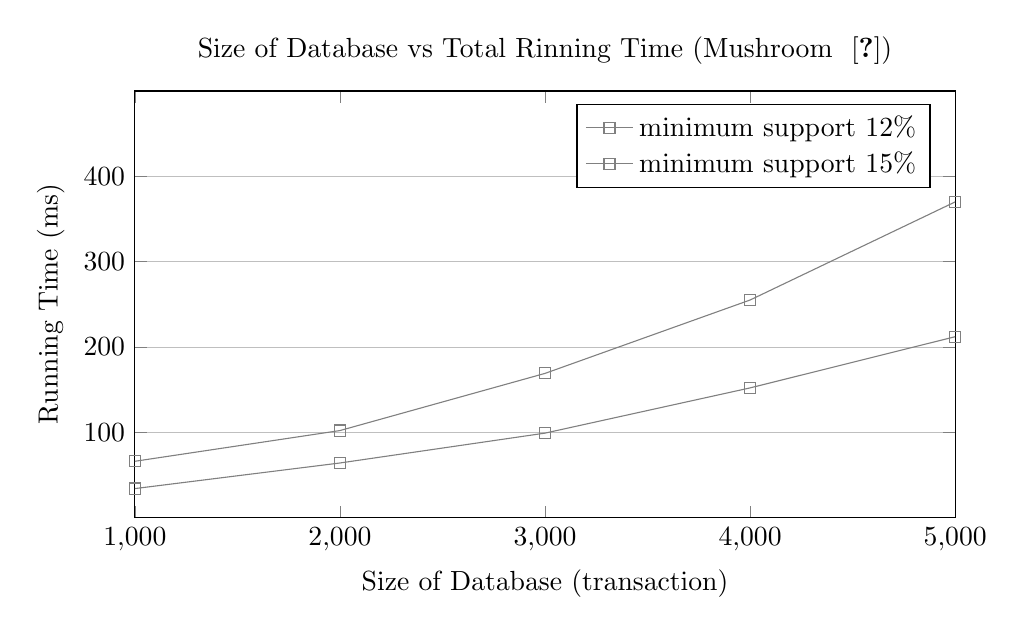
\begin{tikzpicture}
\begin{axis}[
	title={Size of Database vs Total Rinning Time (Mushroom ~\cite{dataset})},
	width=12cm,
	height=7cm,
    xlabel={Size of Database (transaction)},
    ylabel={Running Time (ms)},
    xmin=1000, xmax=5000,
    ymin=0, ymax=500,
    xtick={1000,2000,3000,4000,5000},
    ytick={100,200,300,400},
    legend pos=north east,
    ymajorgrids=true,
    grid style={line width=.2pt,draw=gray!50},
]
 
\addplot[
    solid,color=gray, every mark/.append style={solid, fill=gray}, mark=square
    ]
    coordinates {
		(1000,34)
		(2000,64)
		(3000,99)
		(4000,152)
		(5000,212)

	};
    \addlegendentry{minimum support 12\%}
	
\addplot[
    solid,color=gray, every mark/.append style={solid, fill=gray}, mark=square
    ]
    coordinates {
		(1000,66)
		(2000,102)
		(3000,169)
		(4000,255)
		(5000,370)

	};
    \addlegendentry{minimum support 15\%}

\end{axis}
\end{tikzpicture}
%\end{document}
        \caption{Size of Database vs Runtime for Mushroom Dataset }
        \label{result:g_m_const_tran}
        \end{figure}
        \begin{figure}[h]
        \centering
            %mark = star, diamond, square, otimes
%\documentclass{article}
%\usepackage{pgfplots}
%\usepackage[justification=centering]{caption}
%\pgfplotsset{compat=newest}
%\begin{document}
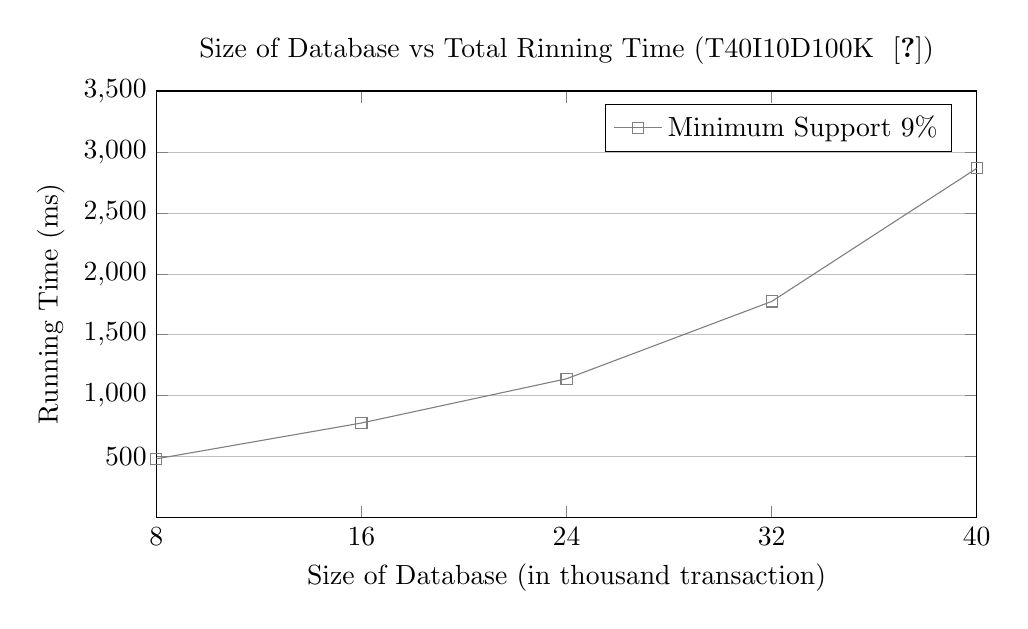
\begin{tikzpicture}
\begin{axis}[
	title={Size of Database vs Total Rinning Time (T40I10D100K ~\cite{dataset})},
	width=12cm,
	height=7cm,
    xlabel={Size of Database (in thousand transaction)},
    ylabel={Running Time (ms)},
    xmin=8, xmax=40,
    ymin=0, ymax=3500,
    xtick={8,16,24,32,40},
    ytick={500,1000,1500,2000,2500,3000,3500},
    legend pos=north east,
    ymajorgrids=true,
    grid style={line width=.2pt,draw=gray!50},
]
 
\addplot[
    solid,color=gray, every mark/.append style={solid, fill=gray}, mark=square
    ]
    coordinates {
			(8,482)
			(16,776)
			(24,1139)
			(32,1773)
			(40,2865)

	};
    \addlegendentry{Minimum Support 9\%}

\end{axis}
\end{tikzpicture}
%\end{document}
        \caption{Size of Database vs Runtime for T40I10D100K Dataset }
        \label{result:g_t10_const_tran}
        \end{figure}
%        \begin{figure}[h]
%        \centering
%            %mark = star, diamond, square, otimes
%\documentclass{article}
%\usepackage{pgfplots}
%\usepackage[justification=centering]{caption}
%\pgfplotsset{compat=newest}
%\begin{document}
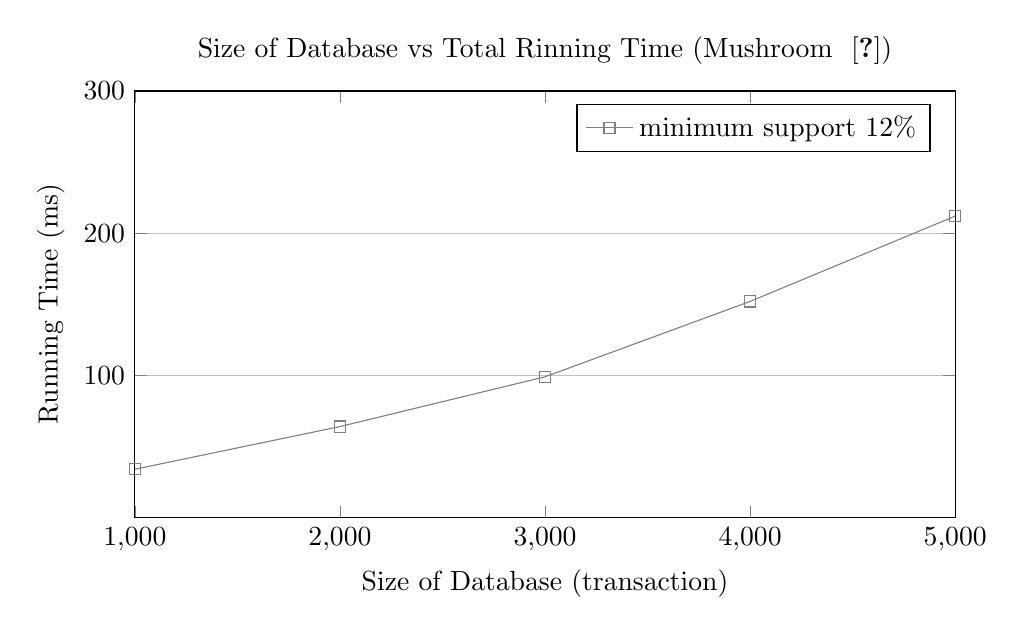
\begin{tikzpicture}
\begin{axis}[
	title={Size of Database vs Total Rinning Time (Mushroom ~\cite{dataset})},
	width=12cm,
	height=7cm,
    xlabel={Size of Database (transaction)},
    ylabel={Running Time (ms)},
    xmin=1000, xmax=5000,
    ymin=0, ymax=300,
    xtick={1000,2000,3000,4000,5000},
    ytick={100,200,300},
    legend pos=north east,
    ymajorgrids=true,
    grid style={line width=.2pt,draw=gray!50},
]
 
\addplot[
    solid,color=gray, every mark/.append style={solid, fill=gray}, mark=square
    ]
    coordinates {
		(1000,34)
		(2000,64)
		(3000,99)
		(4000,152)
		(5000,212)

	};
    \addlegendentry{minimum support 12\%}

\end{axis}
\end{tikzpicture}
%\end{document}
%        \caption{Size of Database vs Runtime for Kosarak Dataset }
%        \label{result:g_k_const_tran}
%        \end{figure}
        %%%%%%%%%%%%%%%%%%%%%%%%%%%%%%%%%%%%%%%%%%%%%%%%%%%%%%%%%%%%%%%%%%%%%%%%%%%%%%%%%%%%%%%%%%%%%%%%%%%%%%%%%%%%%%%%%%%%%%%%%%%%%%%%%%%%%%%%%%%%%%%%%%%%%%%%%%%%%%%%%%%%%%%%%%%%%%%%%%%%%%%%%%%%%%%%%%%%%%%%%%%%%%%%%%%%%%%%%%%%%
%        \begin{figure}[h]
%        \centering
%            %mark = star, diamond, square, otimes
%\documentclass{article}
%\usepackage{pgfplots}
%\usepackage[justification=centering]{caption}
%\pgfplotsset{compat=newest}
%\begin{document}
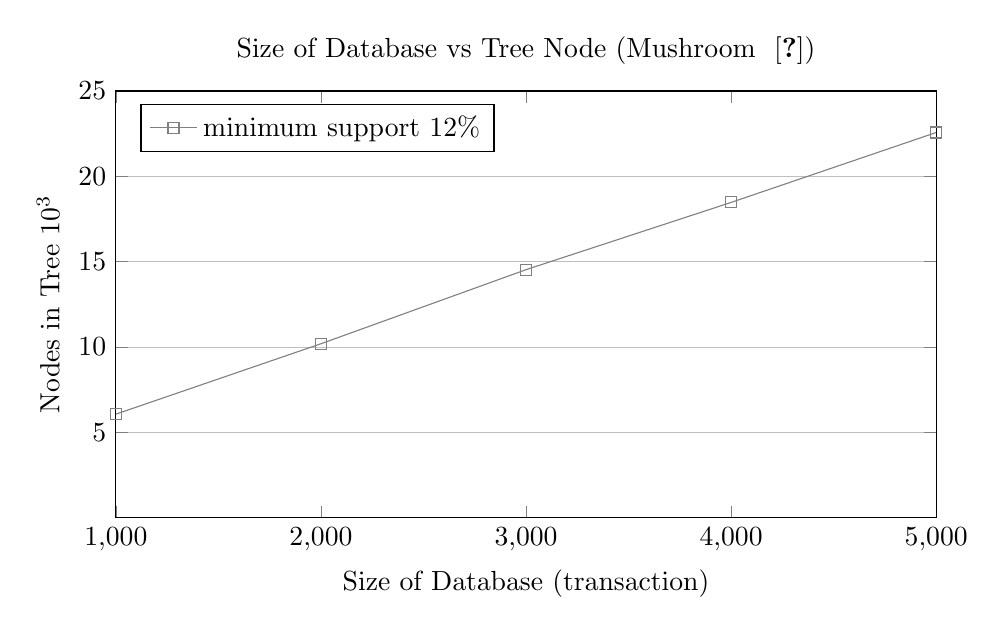
\begin{tikzpicture}
\begin{axis}[
	title={Size of Database vs Tree Node (Mushroom ~\cite{dataset})},
	width=12cm,
	height=7cm,
	xlabel={Size of Database (transaction)},
    ylabel={Nodes in Tree $10^3$},
    xmin=1000, xmax=5000,
    ymin=0, ymax=25,
    xtick={1000,2000,3000,4000,5000},
    ytick={5,10,15,20,25},
    legend pos=north west,
    ymajorgrids=true,
    grid style={line width=.2pt,draw=gray!50},
]
 
\addplot[
    solid,color=gray, every mark/.append style={solid, fill=gray}, mark=square
    ]
    coordinates {
			(1000,6.061 )
			(2000,10.187)
			(3000,14.528)
			(4000,18.469)
			(5000,22.566)


	};
    \addlegendentry{minimum support 12\%}

\end{axis}
\end{tikzpicture}
%\end{document}
%        \caption{Size of Database vs Total Nodes in Tree for Mushroom Dataset }
%        \label{result:g_m_const_tran_mem}
%        \end{figure}
%        \begin{figure}[h]
%        \centering
%            %mark = star, diamond, square, otimes
%\documentclass{article}
%\usepackage{pgfplots}
%\usepackage[justification=centering]{caption}
%\pgfplotsset{compat=newest}
%\begin{document}
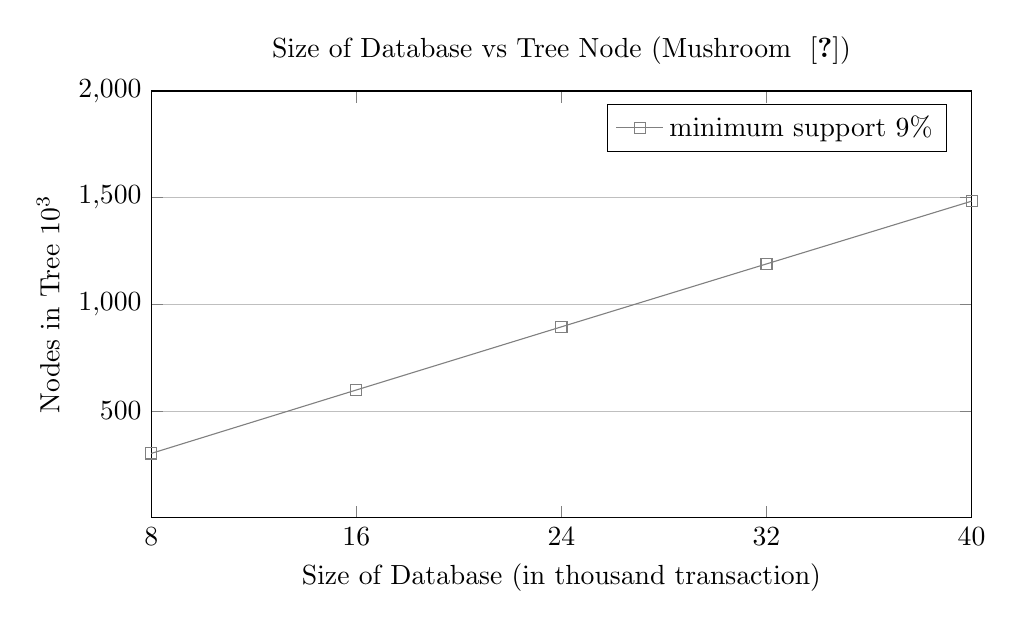
\begin{tikzpicture}
\begin{axis}[
	title={Size of Database vs Tree Node (Mushroom ~\cite{dataset})},
	width=12cm,
	height=7cm,
    xlabel={Size of Database (in thousand transaction)},
    ylabel={Nodes in Tree $10^3$},
    xmin=8, xmax=40,
    ymin=0, ymax=2000,
    xtick={8,16,24,32,40},
    ytick={500,1000,1500,2000},
    legend pos=north east,
    ymajorgrids=true,
    grid style={line width=.2pt,draw=gray!50},
]
 
\addplot[
    solid,color=gray, every mark/.append style={solid, fill=gray}, mark=square
    ]
    coordinates {
			(8,300.856)
			(16,598.221)
			(24,894.225)
			(32,1189.166)
			(40,1483.378)



	};
    \addlegendentry{minimum support 9\%}

\end{axis}
\end{tikzpicture}
%\end{document}
%        \caption{Size of Database vs Total Nodes in Tree for T40I10D100K Dataset }
%        \label{result:g_t10_const_tran_mem}
%        \end{figure}
%        \begin{figure}[h]
%        \centering
%            %mark = star, diamond, square, otimes
%\documentclass{article}
%\usepackage{pgfplots}
%\usepackage[justification=centering]{caption}
%\pgfplotsset{compat=newest}
%\begin{document}
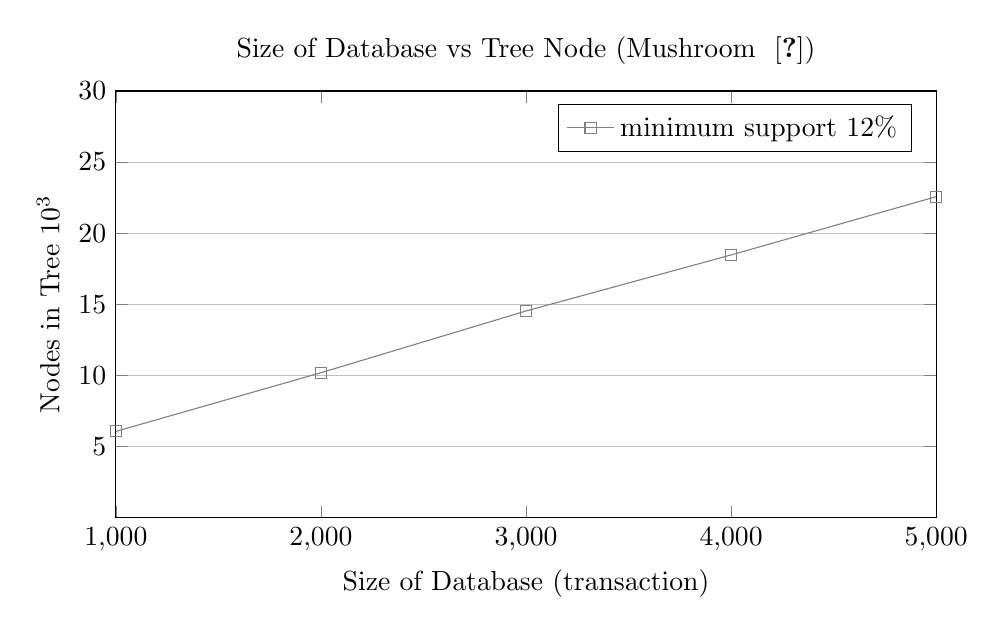
\begin{tikzpicture}
\begin{axis}[
	title={Size of Database vs Tree Node (Mushroom ~\cite{dataset})},
	width=12cm,
	height=7cm,
	xlabel={Size of Database (transaction)},
    ylabel={Nodes in Tree $10^3$},
    xmin=1000, xmax=5000,
    ymin=0, ymax=30,
    xtick={1000,2000,3000,4000,5000},
    ytick={5,10,15,20,25,30},
    legend pos=north east,
    ymajorgrids=true,
    grid style={line width=.2pt,draw=gray!50},
]
 
\addplot[
    solid,color=gray, every mark/.append style={solid, fill=gray}, mark=square
    ]
    coordinates {
			(1000,6.061 )
			(2000,10.187)
			(3000,14.528)
			(4000,18.469)
			(5000,22.566)


	};
    \addlegendentry{minimum support 12\%}

\end{axis}
\end{tikzpicture}
%\end{document}
%        \caption{Size of Database vs Total Nodes in Tree for Kosarak Dataset }
%        \label{result:g_k_const_tran_mem}
%        \end{figure}
%        
		\begin{table}[h]
        \centering
        \begin{tabular}{|c|c|}
        \hline 
       Size of Database        &    Memory (in MB)\\    \hline\hline
        
				1000&0.473\\\hline
				2000&0.795\\\hline
				3000&1.135\\\hline
				4000&1.442\\\hline
				5000&1.762\\\hline
		
            \end{tabular}
        \caption{ Total Memory (in MB) in Tree for Mushroom Dataset}
        \label{result:g_m_const_tran_mem}
        \end{table}
		
		\begin{table}[h]
        \centering
        \begin{tabular}{|c|c|}
        \hline 
       Size of Database       &    Memory (in MB)\\    \hline\hline
        
				8000 &23.504\\\hline
				10000&46.736\\\hline
				24000&69.861\\\hline
				32000&92.903\\\hline
				40000&115.888\\\hline
		
            \end{tabular}
        \caption{ Total Memory (in MB) in Tree for T40I10D100K Dataset}
        \label{result:g_t10_const_tran_mem}
        \end{table}
    \paragraph{Window Size Change Effect}For window size change effect we have experimented our algorithm in the different angle. The experiment shows the window size change effect do not hamper performance and it is consistent. Figure-\ref{result:g_m_const_batch} and figure-\ref{result:g_t10_const_batch} shows effect of window size change effect on mushroom and T40I10D100K dataset.
        %%%%%%%%%%%%%%%%%%%%%%%%%%%%%%%%%%%%%%%%%%%%%%%%%%%%%%%%%%%%%%%%%%%%%%%%%%%%%%%%%%%%%%%%%%%%%%%%%%%%%%%%%%%%%%%%%%%%%%%%%%%%%%%%%%%%%%%%%%%%%%%%%%%%%%%%%%%%%%%%%%%%%%%%%%%%%%%%%%%%%%%%%%%%%%%%%%%%%%%%%%%%%%%%%%%%%%%%%%%%%
        \begin{figure}[h]
        \centering
            %mark = star, diamond, square, otimes
%\documentclass{article}
%\usepackage{pgfplots}
%\usepackage[justification=centering]{caption}
%\pgfplotsset{compat=newest}
%\begin{document}
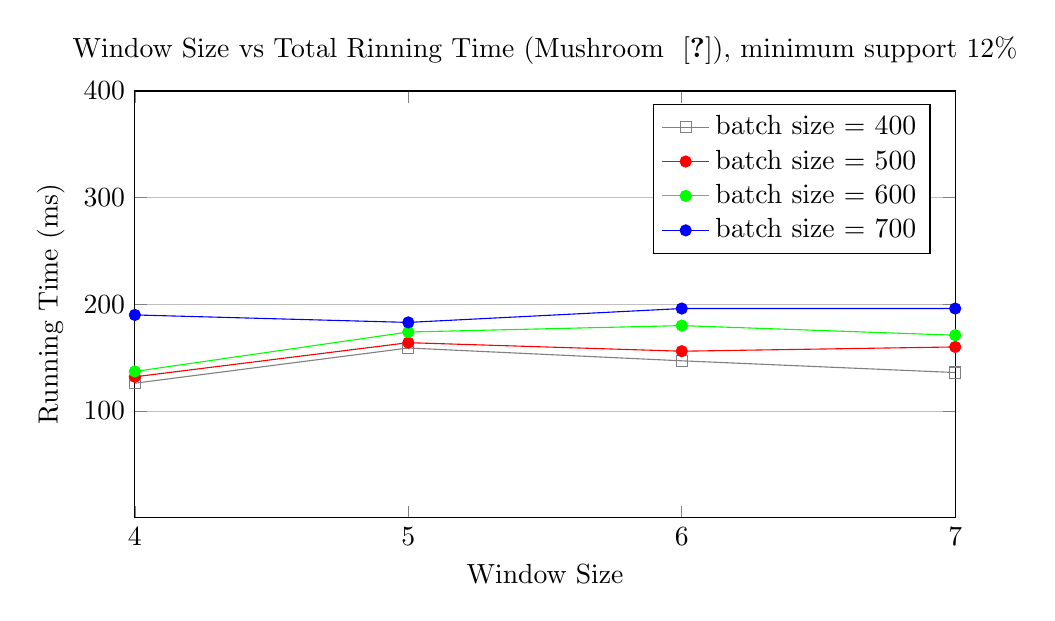
\begin{tikzpicture}
\begin{axis}[
 title={Window Size vs Total Rinning Time (Mushroom ~\cite{dataset}), minimum support 12\%},
 width=12cm,
   height=7cm,
    xlabel={Window Size},
	    ylabel={Running Time (ms)},
    xmin=4, xmax=7,
    ymin=0, ymax=400,
    xtick={4,5,6,7},
    ytick={100,200,300,400},
    legend pos=north east,
    ymajorgrids=true,
    grid style={line width=.2pt,draw=gray!50},
]
 
\addplot[
    solid,color=gray, every mark/.append style={solid, fill=gray}, mark=square
    ]
    coordinates {
			(4,126)			
			(5,159)			
			(6,147)			
			(7,136)
	};
    \addlegendentry{batch size $=$ 400}

	\addplot[
    solid,color=red, every mark/.append style={solid, fill=red}, mark=*
    ]
    coordinates {
			(4,132)			
			(5,164)			
			(6,156)			
			(7,160)
};
    \addlegendentry{batch size $=$ 500}
	

\addplot[
    solid,color=green, every mark/.append style={solid, fill=green}, mark=*
    ]
    coordinates {
			(4,137)			
			(5,174)			
			(6,180)			
			(7,171)
};
    \addlegendentry{batch size $=$ 600}
	
	
\addplot[
    solid,color=blue, every mark/.append style={solid, fill=blue}, mark=*
    ]
    coordinates {
			(4,190)			
			(5,183)			
			(6,196)			
			(7,196)
};
    \addlegendentry{batch size = 700}
\end{axis}
\end{tikzpicture}
%\end{document}
        \caption{Batch Size vs Runtime for Mushroom Dataset }
        \label{result:g_m_const_batch}
        \end{figure}
        \begin{figure}[h]
        \centering
            %mark = star, diamond, square, otimes
%\documentclass{article}
%\usepackage{pgfplots}
%\usepackage[justification=centering]{caption}
%\pgfplotsset{compat=newest}
%\begin{document}
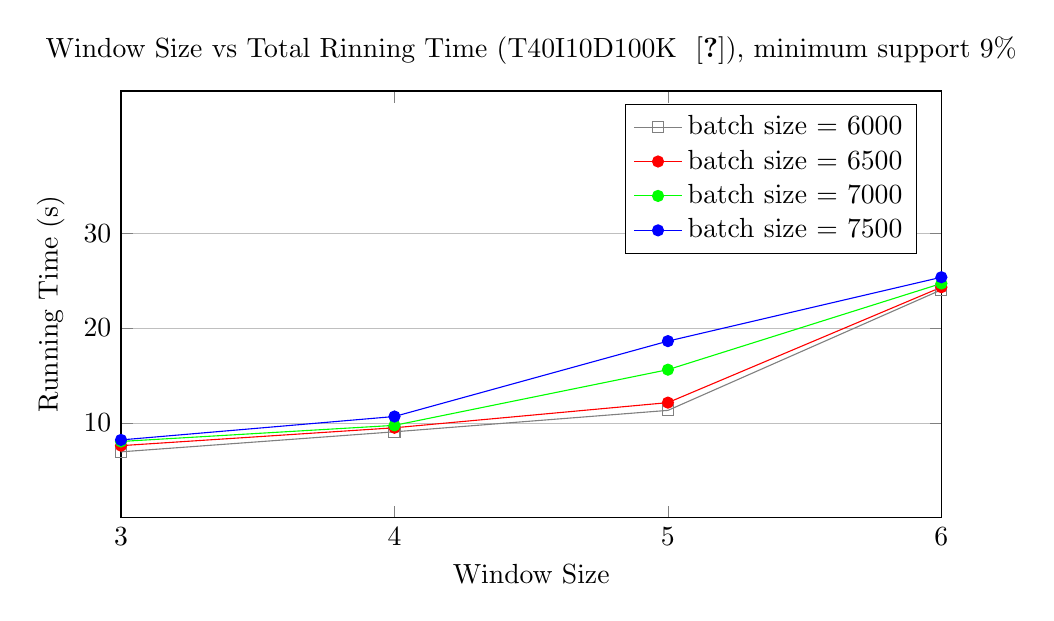
\begin{tikzpicture}
\begin{axis}[
 title={Window Size vs Total Rinning Time (T40I10D100K ~\cite{dataset}), minimum support 9\%},
 width=12cm,
   height=7cm,
    xlabel={Window Size},
    ylabel={Running Time (s)},
    xmin=3, xmax=6,
    ymin=0, ymax=45,
    xtick={3,4,5,6},
    ytick={10,20,30},
    legend pos=north east,
    ymajorgrids=true,
    grid style={line width=.2pt,draw=gray!50},
]
 
\addplot[
    solid,color=gray, every mark/.append style={solid, fill=gray}, mark=square
    ]
    coordinates {
		(3,6.935 )
		(4,9.048 )
		(5,11.308)
		(6,24.026)

	};
    \addlegendentry{batch size $=$ 6000}

	\addplot[
    solid,color=red, every mark/.append style={solid, fill=red}, mark=*
    ]
    coordinates {
		(3,7.587)
		(4,9.473)
		(5,12.126)
		(6,24.299)
};
    \addlegendentry{batch size $=$ 6500}
	

\addplot[
    solid,color=green, every mark/.append style={solid, fill=green}, mark=*
    ]
    coordinates {
		(3,8.030)
		(4,9.729)
		(5,15.602)
		(6,24.690)

};
    \addlegendentry{batch size $=$ 7000}
	
	
\addplot[
    solid,color=blue, every mark/.append style={solid, fill=blue}, mark=*
    ]
    coordinates {
		(3,8.192)
		(4,10.662)
		(5,18.613)
		(6,25.351)
};
    \addlegendentry{batch size $=$ 7500}
\end{axis}
\end{tikzpicture}
%\end{document}
        \caption{Batch Size vs Runtime for T40I10D100K Dataset }
        \label{result:g_t10_const_batch}
        \end{figure}
        %%%%%%%%%%%%%%%%%%%%%%%%%%%%%%%%%%%%%%%%%%%%%%%%%%%%%%%%%%%%%%%%%%%%%%%%%%%%%%%%%%%%%%%%%%%%%%%%%%%%%%%%%%%%%%%%%%%%%%%%%%%%%%%%%%%%%%%%%%%%%%%%%%%%%%%%%%%%%%%%%%%%%%%%%%%%%%%%%%%%%%%%%%%%%%%%%%%%%%%%%%%%%%%%%%%%%%%        
    \paragraph{Batch Size Change Effect}Like batch change effect we also experimented for batch size change effect.For changing batch size in different volume the result we find is consistent. For constant window and variable batches we have simulated our proposed algorithms. Figure-\ref{result:g_m_const_batch} and figure-\ref{result:g_t10_const_batch} shows effect of batch size change effect on mushroom and T40I10D100K dataset.
        \begin{figure}[h]
        \centering
            %mark = star, diamond, square, otimes
%\documentclass{article}
%\usepackage{pgfplots}
%\usepackage[justification=centering]{caption}
%\pgfplotsset{compat=newest}
%\begin{document}
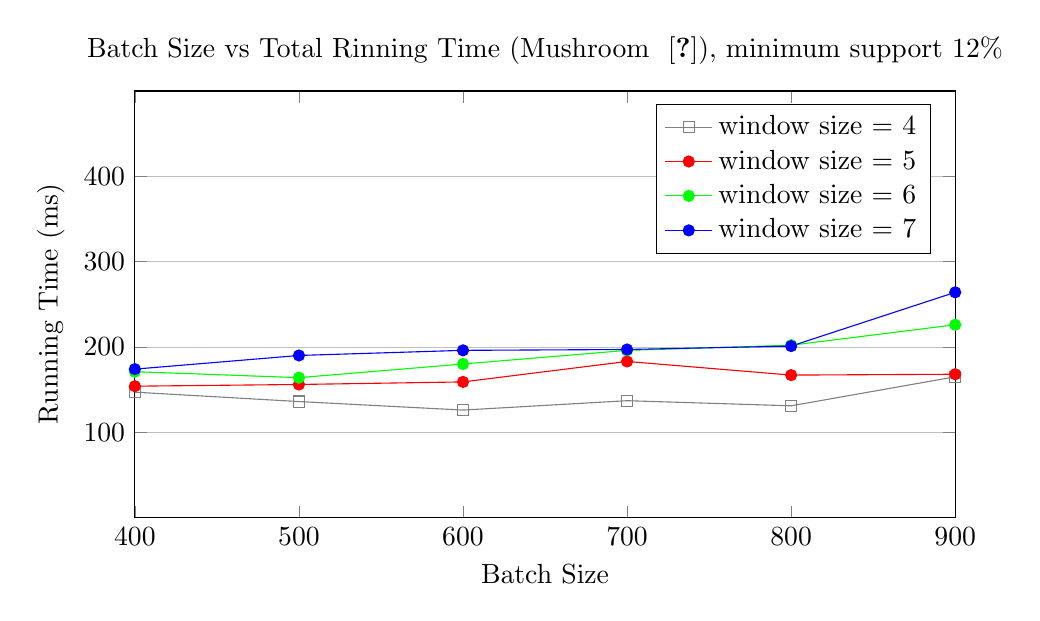
\begin{tikzpicture}
\begin{axis}[
 title={Batch Size vs Total Rinning Time (Mushroom ~\cite{dataset}), minimum support 12\%},
 width=12cm,
   height=7cm,
    xlabel={Batch Size},
    ylabel={Running Time (ms)},
    xmin=400, xmax=900,
    ymin=0, ymax=500,
    xtick={400,500,600,700,800,900},
    ytick={100,200,300,400},
    legend pos=north east,
    ymajorgrids=true,
    grid style={line width=.2pt,draw=gray!50},
]
 
\addplot[
    solid,color=gray, every mark/.append style={solid, fill=gray}, mark=square
    ]
    coordinates {
			(400,147)
			(500,136)
			(600,126)
			(700,137)
			(800,131)
			(900,165)
	};
    \addlegendentry{window size $=$ 4}

	\addplot[
    solid,color=red, every mark/.append style={solid, fill=red}, mark=*
    ]
    coordinates {
			(400,154)
			(500,156)
			(600,159)
			(700,183)
			(800,167)
			(900,168)
};
    \addlegendentry{window size $=$ 5}
	

\addplot[
    solid,color=green, every mark/.append style={solid, fill=green}, mark=*
    ]
    coordinates {
			(400,171)
			(500,164)
			(600,180)
			(700,196)
			(800,202)
			(900,226)
};
    \addlegendentry{window size $=$ 6}
	
	
\addplot[
    solid,color=blue, every mark/.append style={solid, fill=blue}, mark=*
    ]
    coordinates {
			(400,174)
			(500,190)
			(600,196)
			(700,197)
			(800,201)
			(900,264)
};
    \addlegendentry{window size = 7}
\end{axis}
\end{tikzpicture}
%\end{document}
        \caption{Window Size vs Runtime for Mushroom Dataset }
        \label{result:g_m_const_win}
        \end{figure}
        \begin{figure}[h]
        \centering
            %mark = star, diamond, square, otimes
%\documentclass{article}
%\usepackage{pgfplots}
%\usepackage[justification=centering]{caption}
%\pgfplotsset{compat=newest}
%\begin{document}
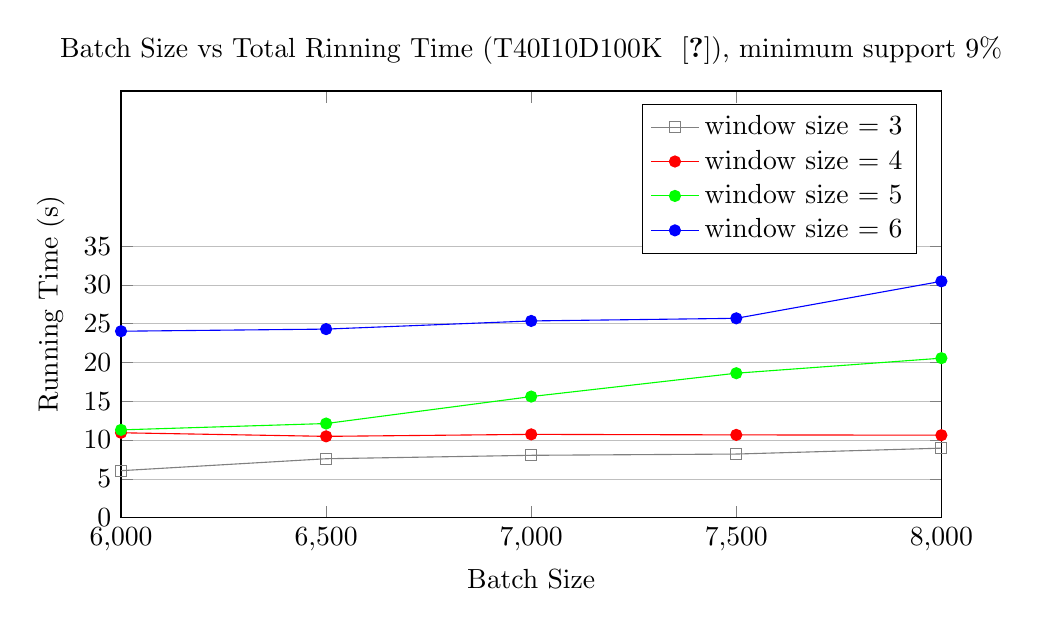
\begin{tikzpicture}
\begin{axis}[
 title={Batch Size vs Total Rinning Time (T40I10D100K ~\cite{dataset}), minimum support 9\%},
 width=12cm,
   height=7cm,
    xlabel={Batch Size},
    ylabel={Running Time (s)},
    xmin=6000, xmax=8000,
    ymin=0, ymax=55,
    xtick={6000,6500,7000,7500,8000},
    ytick={0,5,10,15,20,25,30,35},
    legend pos=north east,
    ymajorgrids=true,
    grid style={line width=.2pt,draw=gray!50},
]
 
\addplot[
    solid,color=gray, every mark/.append style={solid, fill=gray}, mark=square
    ]
    coordinates {
		(6000,6.048)
		(6500,7.587 )
		(7000,8.030 )
		(7500,8.192 )
		(8000,8.951 )
	};
    \addlegendentry{window size $=$ 3}

	\addplot[
    solid,color=red, every mark/.append style={solid, fill=red}, mark=*
    ]
    coordinates {
		(6000,10.935)
		(6500,10.473)
		(7000,10.729)
		(7500,10.662)
		(8000,10.625)

};
    \addlegendentry{window size $=$ 4}
	

\addplot[
    solid,color=green, every mark/.append style={solid, fill=green}, mark=*
    ]
    coordinates {
		(6000,11.308)
		(6500,12.126)
		(7000,15.602)
		(7500,18.613)
		(8000,20.552)

};
    \addlegendentry{window size $=$ 5}
	
	
\addplot[
    solid,color=blue, every mark/.append style={solid, fill=blue}, mark=*
    ]
    coordinates {
		(6000,24.026)
		(6500,24.299)
		(7000,25.351)
		(7500,25.690)
		(8000,30.460)

};
    \addlegendentry{window size $=$ 6}
\end{axis}
\end{tikzpicture}
%\end{document}
        \caption{Window Size vs Runtime for T40I10D100K Dataset }
        \label{result:g_t10_const_win}
        \end{figure}
        %%%%%%%%%%%%%%%%%%%%%%%%%%%%%%%%%%%%%%%%%%%%%%%%%%%%%%%%%%%%%%%%%%%%%%%%%%%%%%%%%%%%%%%%%%%%%%%%%%%%%%%%%%%%%%%%%%%%%%%%%%%%%%%%%%%%%%%%%%%%%%%%%%%%%%%%%%%%%%%%%%%%%%%%%%%%%%%%%%%%%%%%%%%%%%%%%%%%%%%%%%%%%%%%%%%%%%%%%%%%%
\clearpage
%%%%%%%%%%%%%%%%%%%%%%%%%%%%%%%%%%%%%%%%%%%%%%%%%%%%%%%%%%%%%%%%%%%%%%%%%%%%%%%%%%%%%%%%%%%%%%%%%%%%%%%%%%%%%%%%%%%%%%%%%%%%%%%%%%%%%%%%%%%%%%%%%%%%%%%%%%%%%%%%%%%%%%%%%%%%%%%%%%%%%%%%%%%%%%%%%%%%%%%%%%%%%%%%%%%%%%%%%%%%%        
\subsection{Comparison With Existing Approaches}
Here now we have compared our proposed approach with existing system. We have choose SUF-growth ~\cite{suf_growth}  for comparison. This algorithm is perfectly fit for uncertain stream data mining. UF-streaming also designed for mining frequent patterns from uncertain stream but in ~\cite{suf_growth} it has been proved that in all criteria (runtime, memory and correctness) SUF-growth ~\cite{suf_growth} is better than UF-streaming ~\cite{suf_growth}. We have experimented for both runtime performance and memory efficiency. The result has described below:
    \subsubsection{Runtime Comparison}
    Runtime comparison has been experimented and the in the result we found is consistent and we have gained runtime efficiency for both dense and sparse dataset. For mushroom dataset our approach's total tree construction time , total mining time and total time has been compared with SUF-growth ~\cite{suf_growth}'s tree construction time and mining time and total time. Figure-\ref{result:g_m_tree_construction_total}, figure-\ref{result:g_m_mining_total} and figure-\ref{result:g_m_total} shows the result graph. As mushroom is a dense database we gain much more in run time. For dense characteristic the constructed \emph{US-tree} is very much compact and moreover when mining compact tree the mining time surprisingly decreases that affect the total time. Figure-\ref{result:g_t10_tree_construction_total}, figure-\ref{result:g_t10_mining_total} and figure-\ref{result:g_t10_total} shows same comparison for T40I10D100K dataset . The graphs shows that our algorithm works correctly for sparse dataset too. Figure-\ref{result:g_chess_tree_construction_total}, figure-\ref{result:g_chess_mining_total} and figure-\ref{result:g_chess_total} shows tree construction time, mining time and total time for chess dataset. Kosarak is very large and real-life data set. This is web click database. This database is sparse and very much large. \ref{result:g_k_tree_construction_total}, figure-\ref{result:g_k_mining_total} and figure-\ref{result:g_k_total} shows the effect of changing minimum support effect corresponding to tree construction time, mining time and total time. This one is dense dataset and the result is consistent, efficient and also scalable.
            \begin{figure}[h]
            \centering
                %%mark = star, diamond, square, otimes
%\documentclass{article}
%\usepackage{pgfplots}
%\usepackage[justification=centering]{caption}
%\pgfplotsset{compat=newest}
%\begin{document}
\begin{figure}
\centering

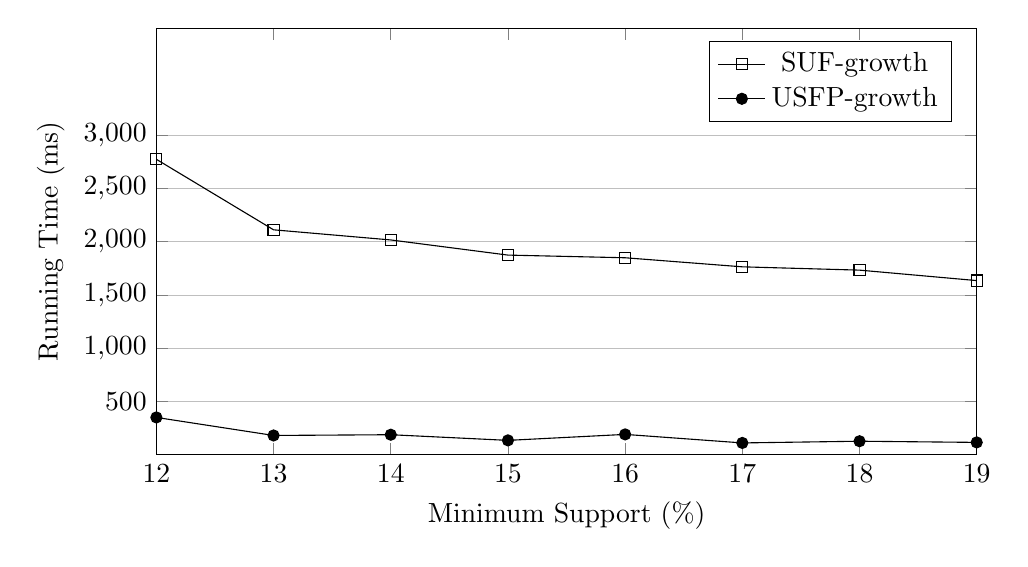
\begin{tikzpicture}
\begin{axis}[
 width=12cm,
   height=7cm,
    xlabel={Minimum Support (\%) },
    ylabel={Running Time (ms)},
    xmin=12, xmax=19,
    ymin=0, ymax=4000,
    xtick={12,13,14,15,16,17,18,19},
    ytick={500,1000,1500,2000,2500,3000},
    legend pos=north east,
    ymajorgrids=true,
    grid style={line width=.2pt,draw=gray!50},
]
 
\addplot[
    solid, every mark/.append style={solid, fill=gray}, mark=square
    ]
    coordinates {
	(12,2771)
	(13,2110)
	(14,2015)
	(15,1873)
	(16,1848)
	(17,1763)
	(18,1732)
	(19,1634)
	};
    \addlegendentry{SUF-growth}
\addplot[
    solid, every mark/.append style={solid, fill=black}, mark=*
    ]
    coordinates {
	(12,351)
	(13,182)
	(14,189)
	(15,136)
	(16,192)
	(17,112)
	(18,128)
	(19,117)
};
    \addlegendentry{USFP-growth}
 
\end{axis}
\end{tikzpicture}
%\caption{Total Tree Construction Time vs Minimum Suppport (\%) \\(Window Size = 4, Frame Size = 650) for mushroom database}
\label{result:mushroom_tree_total}
\end{figure}
%\end{document}
            \caption{Total Tree Construction Time vs Minimum Support (\%) for Mushroom Dataset }
            \label{result:g_m_tree_construction_total}
            \end{figure}
            
            \begin{figure}[h]
            \centering
                %mark = star, diamond, square, otimes
\documentclass{article}
\usepackage{pgfplots}
\usepackage[justification=centering]{caption}
\pgfplotsset{compat=newest}
\begin{document}
\begin{figure}
\centering

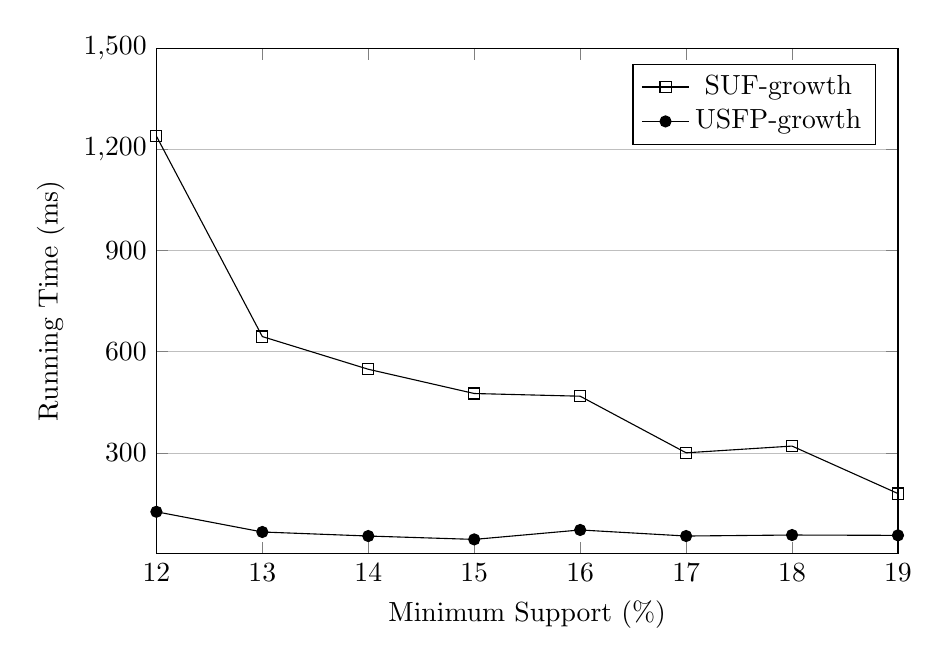
\begin{tikzpicture}
\begin{axis}[
 width=11cm,
   height=8cm,
    xlabel={Minimum Support (\%) },
    ylabel={Running Time (ms)},
    xmin=12, xmax=19,
    ymin=0, ymax=1500,
    xtick={12,13,14,15,16,17,18,19},
    ytick={300,600,900,1200,1500,2000},
    legend pos=north east,
    ymajorgrids=true,
    grid style={line width=.2pt,draw=gray!50},
]
 
\addplot[
    solid, every mark/.append style={solid, fill=gray}, mark=square
    ]
    coordinates {
	(12,1240)
	(13,645)
	(14,548)
	(15,476)
	(16,468)
	(17,300)
	(18,320)
	(19,179)
};
    \addlegendentry{SUF-growth}
\addplot[
    solid, every mark/.append style={solid, fill=black}, mark=*
    ]
    coordinates {
	(12,125)
	(13,65 )
	(14,53 )
	(15,43 )
	(16,71 )
	(17,53 )
	(18,56 )
	(19,55 )
};
    \addlegendentry{USFP-growth}
 
\end{axis}
\end{tikzpicture}
\caption{Total Tree Mining vs Minimum Suppport (\%) \\(Window Size = 4, Frame Size = 650) for mushroom database}
\label{result:mushroom_total}
\end{figure}
\end{document}
            \caption{Total Tree Mining Time vs Minimum Support (\%) for Mushroom Dataset }
            \label{result:g_m_mining_total}
            \end{figure}
            \begin{figure}[h]
            \centering
                %%mark = star, diamond, square, otimes
%\documentclass{article}
%\usepackage{pgfplots}
%\usepackage[justification=centering]{caption}
%\pgfplotsset{compat=newest}
%\begin{document}
\begin{figure}
\centering

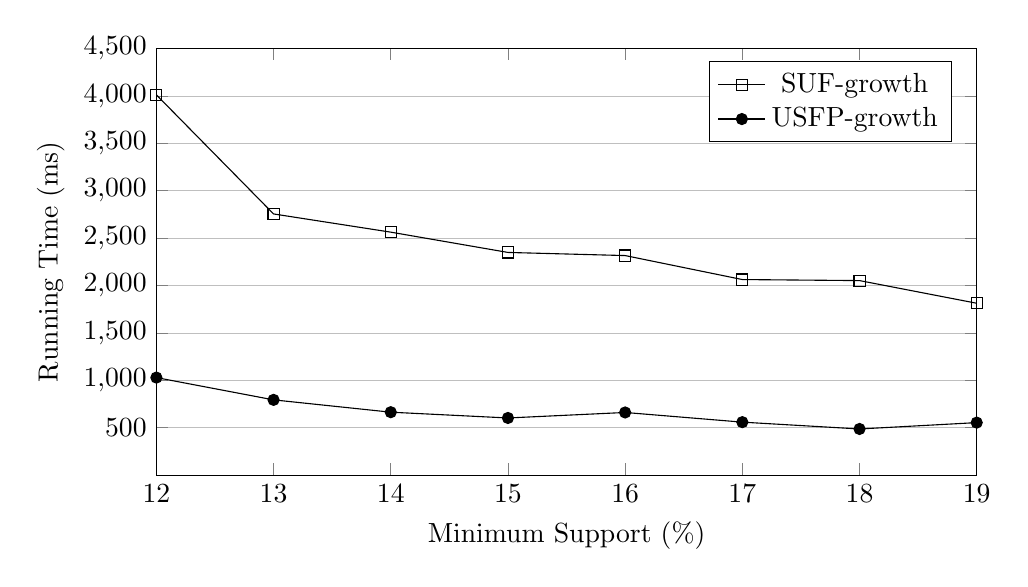
\begin{tikzpicture}
\begin{axis}[
 width=12cm,
   height=7cm,
    xlabel={Minimum Support (\%) },
    ylabel={Running Time (ms)},
    xmin=12, xmax=19,
    ymin=0, ymax=4500,
    xtick={12,13,14,15,16,17,18,19},
    ytick={500,1000,1500,2000,2500,3000,3500,4000,4500},
    legend pos=north east,
    ymajorgrids=true,
    grid style={line width=.2pt,draw=gray!50},
]
 
\addplot[
    solid, every mark/.append style={solid, fill=gray}, mark=square
    ]
    coordinates {
	(12,4011)
	(13,2755)
	(14,2563)
	(15,2349)
	(16,2316)
	(17,2063)
	(18,2052)
	(19,1813)
};
    \addlegendentry{SUF-growth}
\addplot[
    solid, every mark/.append style={solid, fill=black}, mark=*
    ]
    coordinates {
	(12,1029)
	(13,794)
	(14,664)
	(15,603)
	(16,661)
	(17,559)
	(18,487)
	(19,554)
};
    \addlegendentry{USFP-growth}
 
\end{axis}
\end{tikzpicture}
caption{Total Time (Tree Construction + Mining + False Positive Reduction) vs Minimum Suppport (\%) ( Window Size = 4, Frame Size = 650 ) for mushroom database}
\label{result:mushroom_total}
\end{figure}
%\end{document}
            \caption{Runtime vs Minimum Support (\%) for Mushroom Dataset }
            \label{result:g_m_total}
            \end{figure}
            \begin{figure}[h]
            \centering
                %%mark = star, diamond, square, otimes
%\documentclass{article}
%\usepackage{pgfplots}
%\usepackage[justification=centering]{caption}
%\pgfplotsset{compat=newest} 	title={\parbox{\linewidth}{\centering Total Tree Construction Time vs Minimum Suppport (\%) for T40I10D100K ~\cite{dataset}, Window Size = 5, Frame Size = 7000}},
%\begin{document}
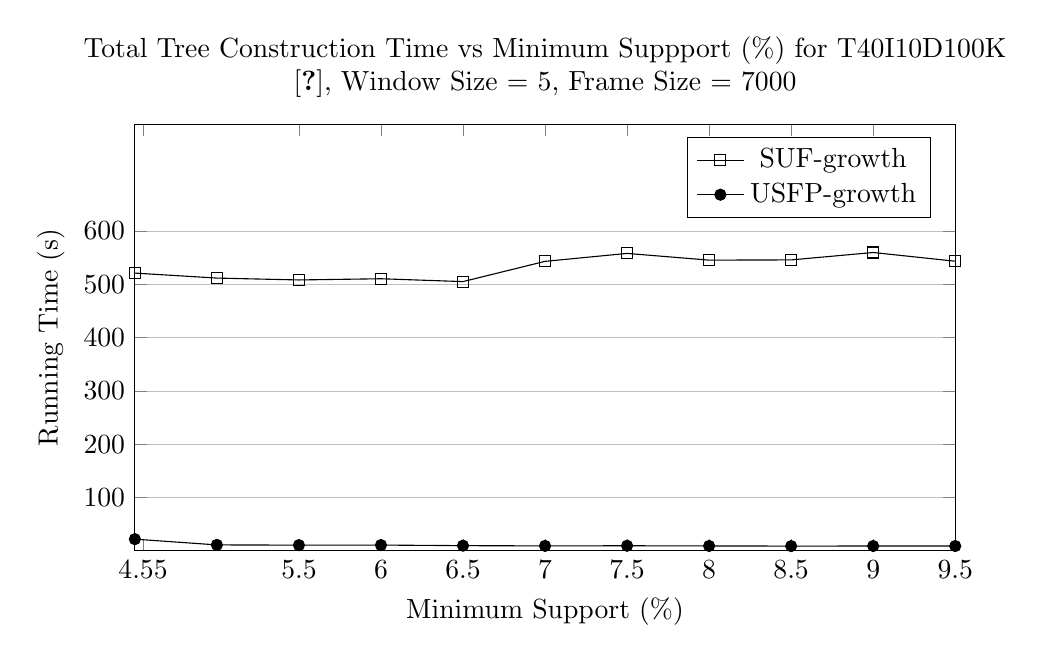
\begin{tikzpicture}
	\begin{axis}[
	title={\parbox{\linewidth}{\centering Total Tree Construction Time vs Minimum Suppport (\%) for T40I10D100K ~\cite{dataset}, Window Size = 5, Frame Size = 7000}},
	width=12cm,
	height=7cm,
    xlabel={Minimum Support (\%) },
    ylabel={Running Time (s)},
    xmin=4.5, xmax=9.5,
    ymin=0, ymax=800,
    xtick={4.55,5.5,6,6.5,7,7.5,8,8.5,9,9.5},
    ytick={100,200,300,400,500,600},
    legend pos=north east,
    ymajorgrids=true,
    grid style={line width=.2pt,draw=gray!50},
]
 
\addplot[
    solid, every mark/.append style={solid, fill=gray}, mark=square
    ]
    coordinates {
			(4.5,520.723)
			(5  ,511.365)
			(5.5,507.854)
			(6  ,510.12 )
			(6.5,504.767)
			(7  ,542.742)
			(7.5,557.633)
			(8  ,545.039)
			(8.5,545.444)
			(9  ,559.335)
			(9.5,542.996)

	};
    \addlegendentry{SUF-growth}
\addplot[
    solid, every mark/.append style={solid, fill=black}, mark=*
    ]
    coordinates {
		(4.5,21.814)
		(5  ,11.035)
		(5.5,10.601)
		(6  ,10.723)
		(6.5,9.646 )
		(7  ,9.177 )
		(7.5,9.427 )
		(8  ,9.092 )
		(8.5,8.8   )
		(9  ,8.95  )
		(9.5,8.883 )

};
    \addlegendentry{USFP-growth}
 
\end{axis}
\end{tikzpicture}
%\end{document}
            \caption{Total Tree Construction Time vs Minimum Support (\%) for T40I10D100K Dataset }
            \label{result:g_t10_tree_construction_total}
            \end{figure}
            
            \begin{figure}[h]
            \centering
                %%%mark = star, diamond, square, otimes
%\documentclass{article}
%\usepackage{pgfplots}
%\usepackage[justification=centering]{caption}
%\pgfplotsset{compat=newest}
%\begin{document}
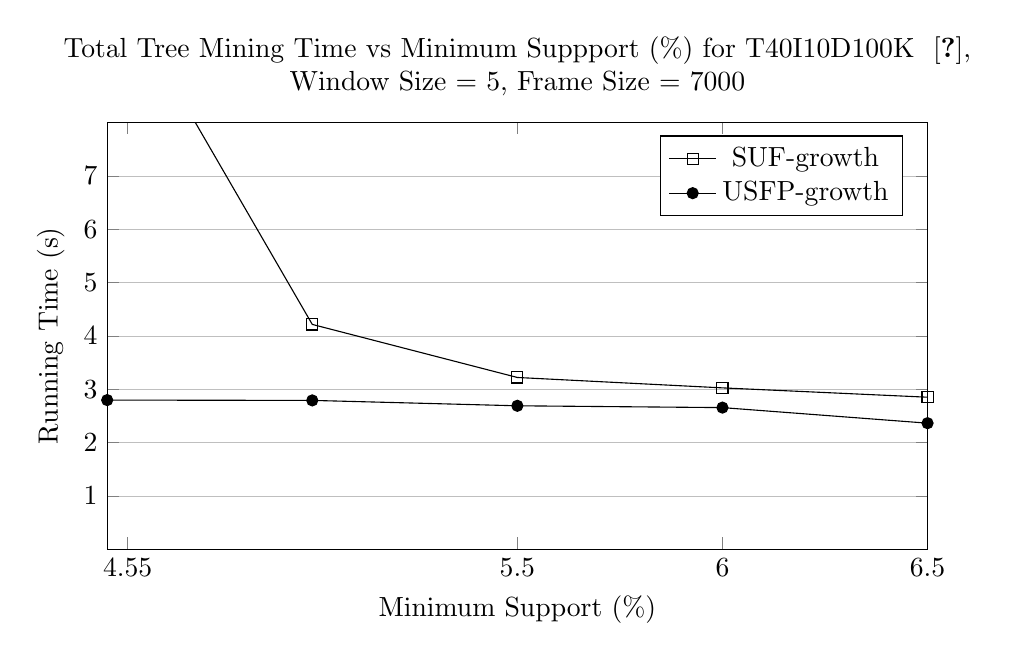
\begin{tikzpicture}
\begin{axis}[
	title={\parbox{\linewidth}{\centering Total Tree Mining Time vs Minimum Suppport (\%) for T40I10D100K ~\cite{dataset}, Window Size = 5, Frame Size = 7000}},
	width=12cm,
	height=7cm,
    xlabel={Minimum Support (\%) },
    ylabel={Running Time (s)},
    xmin=4.5, xmax=6.5,
    ymin=0, ymax=8,
    xtick={4.55,5.5,6,6.5},
    ytick={1,2,3,4,5,6,7},
    legend pos=north east,
    ymajorgrids=true,
    grid style={line width=.2pt,draw=gray!50},
]
 
\addplot[
    solid, every mark/.append style={solid, fill=gray}, mark=square
    ]
    coordinates {
			(4.5,10.856)
			(5  ,4.216 )
			(5.5,3.221 )
			(6  ,3.026 )
			(6.5,2.851 )


};
    \addlegendentry{SUF-growth}
\addplot[
    solid, every mark/.append style={solid, fill=black}, mark=*
    ]
    coordinates {
			(4.5,  2.797)
			(5  , 2.791)
			(5.5,2.69 )
			(6  ,2.656 )
			(6.5,2.364 )


};
    \addlegendentry{USFP-growth}
 
\end{axis}
\end{tikzpicture}
%\end{document}
            \caption{Total Tree Mining Time vs Minimum Support (\%) for T40I10D100K Dataset }
            \label{result:g_t10_mining_total}
            \end{figure}
            
            \begin{figure}[h]
            \centering
                %%%mark = star, diamond, square, otimes
%\documentclass{article}
%\usepackage{pgfplots}
%\usepackage[justification=centering]{caption}
%\pgfplotsset{compat=newest}
%\begin{document}
\begin{figure}[!h]
\centering

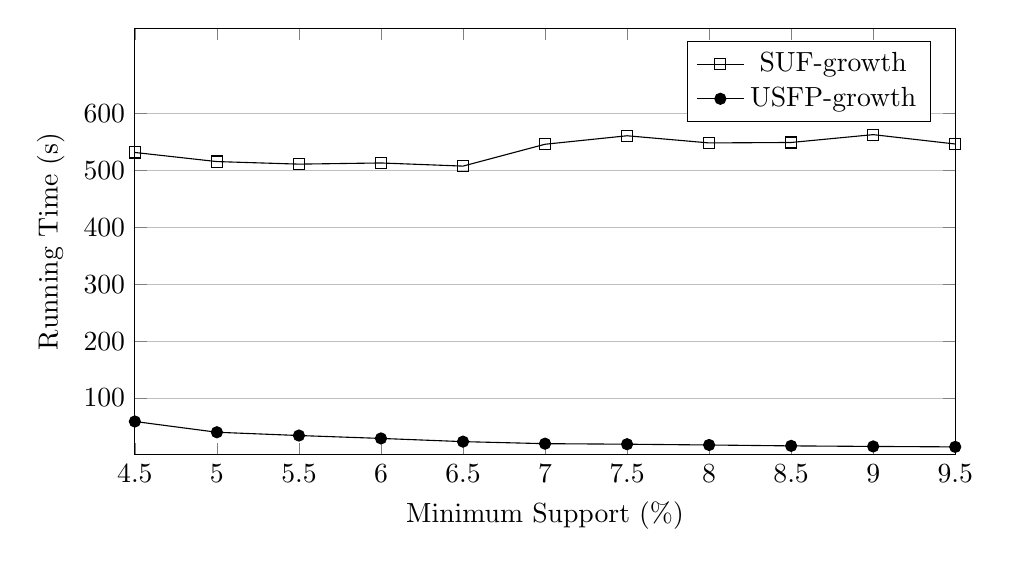
\begin{tikzpicture}
\begin{axis}[
 width=12cm,
   height=7cm,
    xlabel={Minimum Support (\%) },
    ylabel={Running Time (s)},
    xmin=4.5, xmax=9.5,
    ymin=0, ymax=750,
    xtick={4.5,5,5.5,6,6.5,7,7.5,8,8.5,9,9.5},
    ytick={100,200,300,400,500,600},
    legend pos=north east,
    ymajorgrids=true,
    grid style={line width=.2pt,draw=gray!50},
]
 
\addplot[
    solid, every mark/.append style={solid, fill=gray}, mark=square
    ]
    coordinates {
			(4.5,531.579)
			(5  ,515.581)
			(5.5,511.075)
			(6  ,513.146)
			(6.5,507.618)
			(7  ,546.032)
			(7.5,560.952)
			(8  ,548.354)
			(8.5,549.139)
			(9  ,562.928)
			(9.5,546.47 )

};
    \addlegendentry{SUF-growth}
\addplot[
    solid, every mark/.append style={solid, fill=black}, mark=*
    ]
    coordinates {
			(4.5,58.652)
			(5  ,39.735)
			(5.5,33.993)
			(6  ,28.892)
			(6.5,23.262)
			(7  ,19.669)
			(7.5,18.735)
			(8  ,17.355)
			(8.5,15.785)
			(9  ,14.803)
			(9.5,14.013)

};
    \addlegendentry{USFP-growth}
 
\end{axis}
\end{tikzpicture}
\caption{Total Time (Tree Construction + Mining + False Positive Reduction) vs Minimum Suppport (\%) \\(Window Size = 5, Frame Size = 7000) for T40I10D100K database}
\label{result:t10_total}
\end{figure}
%\end{document}
            \caption{Runtime vs Minimum Support (\%) for T40I10D100K Dataset }
            \label{result:g_t10_total}
            \end{figure}
    
            \begin{figure}[h]
            \centering
                %%mark = star, diamond, square, otimes
%\documentclass{article}
%\usepackage{pgfplots}
%\usepackage[justification=centering]{caption}
%\pgfplotsset{compat=newest}
%\begin{document} 
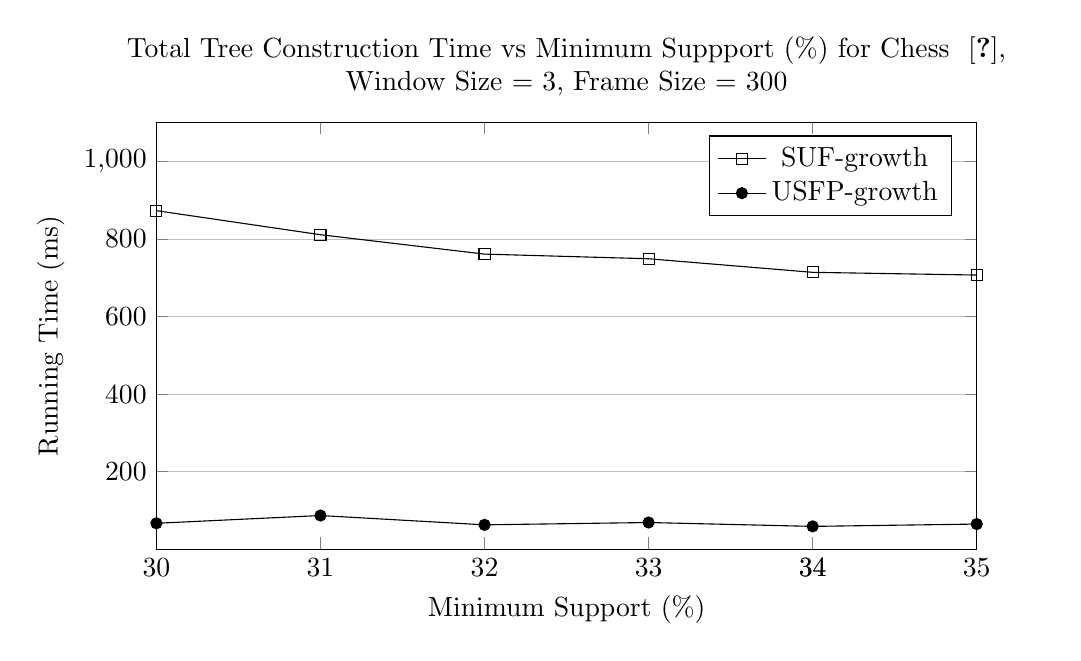
\begin{tikzpicture}
\begin{axis}[
	title={\parbox{\linewidth}{\centering Total Tree Construction Time vs Minimum Suppport (\%) for Chess ~\cite{dataset}, Window Size = 3, Frame Size = 300}},
	width=12cm,
	height=7cm,
    xlabel={Minimum Support (\%) },
    ylabel={Running Time (ms)},
    xmin=30, xmax=35,
    ymin=0, ymax=1100,
    xtick={30,31,32,33,34,34,35},
    ytick={200,400,600,800,1000},
    legend pos=north east,
    ymajorgrids=true,
    grid style={line width=.2pt,draw=gray!50},
]
 
\addplot[
    solid, every mark/.append style={solid, fill=gray}, mark=square
    ]
    coordinates {
			(30,873)
			(31,811)
			(32,761)
			(33,749)
			(34,714)
			(35,707)

	};
    \addlegendentry{SUF-growth}
\addplot[
    solid, every mark/.append style={solid, fill=black}, mark=*
    ]
    coordinates {
			(30,67)
			(31,87)
			(32,63)
			(33,69)
			(34,59)
			(35,65)

};
    \addlegendentry{USFP-growth}
 
\end{axis}
\end{tikzpicture}
%\end{document}
            \caption{Total Tree Construction Time vs Minimum Support (\%) for Chess Dataset }
            \label{result:g_chess_tree_construction_total}
            \end{figure}
            
            \begin{figure}[h]
            \centering
                %%mark = star, diamond, square, otimes
%\documentclass{article}
%\usepackage{pgfplots}
%\usepackage[justification=centering]{caption}
%\pgfplotsset{compat=newest}
%\begin{document}
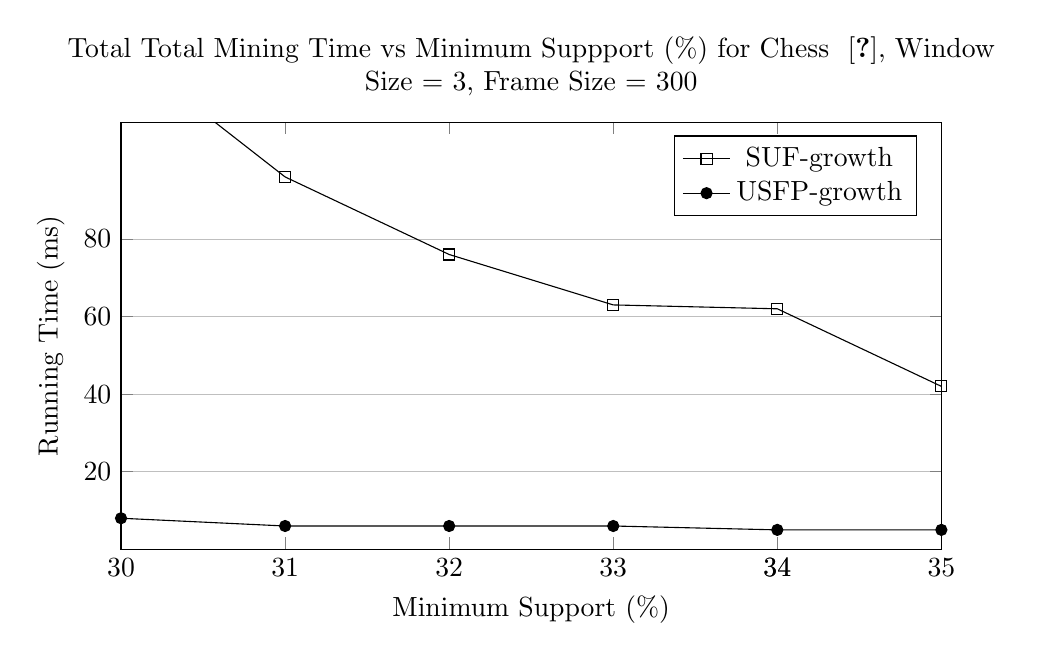
\begin{tikzpicture}
\begin{axis}[
	title={\parbox{\linewidth}{\centering Total Total Mining Time vs Minimum Suppport (\%) for Chess ~\cite{dataset}, Window Size = 3, Frame Size = 300}},
	width=12cm,
	height=7cm,
    xlabel={Minimum Support (\%) },
    ylabel={Running Time (ms)},
    xmin=30, xmax=35,
    ymin=0, ymax=110,
    xtick={30,31,32,33,34,34,35},
    ytick={20,40,60,80},
    legend pos=north east,
    ymajorgrids=true,
    grid style={line width=.2pt,draw=gray!50},
]
 
\addplot[
    solid, every mark/.append style={solid, fill=gray}, mark=square
    ]
    coordinates {
			(30,129)
			(31,96)
			(32,76)
			(33,63)
			(34,62)
			(35,42)

};
    \addlegendentry{SUF-growth}
\addplot[
    solid, every mark/.append style={solid, fill=black}, mark=*
    ]
    coordinates {
			(30,8)
			(31,6)
			(32,6)
			(33,6)
			(34,5)
			(35,5)

};
    \addlegendentry{USFP-growth}
 
\end{axis}
\end{tikzpicture}
%\end{document}
            \caption{Total Tree Mining Time vs Minimum Support (\%) for Chess Dataset }
            \label{result:g_chess_mining_total}
            \end{figure}
            
            \begin{figure}[h]
            \centering
                %%mark = star, diamond, square, otimes
%\documentclass{article}
%\usepackage{pgfplots}
%\usepackage[justification=centering]{caption}
%\pgfplotsset{compat=newest}
%\begin{document}
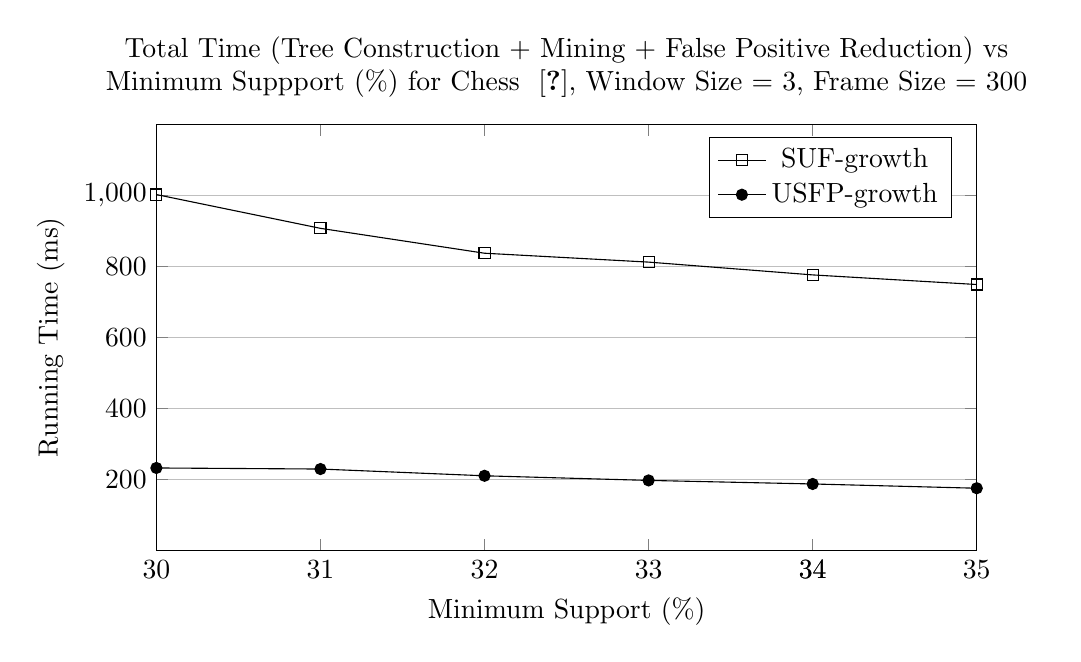
\begin{tikzpicture}
\begin{axis}[
	title={\parbox{\linewidth}{\centering Total Time (Tree Construction + Mining + False Positive Reduction) vs Minimum Suppport (\%) for Chess ~\cite{dataset}, Window Size = 3, Frame Size = 300}},
	width=12cm,
	height=7cm,
    xlabel={Minimum Support (\%) },
    ylabel={Running Time (ms)},
    xmin=30, xmax=35,
    ymin=0, ymax=1200,
    xtick={30,31,32,33,34,34,35},
    ytick={200,400,600,800,1000},
    legend pos=north east,
    ymajorgrids=true,
    grid style={line width=.2pt,draw=gray!50},
]
 
\addplot[
    solid, every mark/.append style={solid, fill=gray}, mark=square
    ]
    coordinates {
			(30,1002)
			(31,907)
			(32,837)
			(33,812)
			(34,776)
			(35,749)
};
    \addlegendentry{SUF-growth}
\addplot[
    solid, every mark/.append style={solid, fill=black}, mark=*
    ]
    coordinates {
			(30,233)
			(31,230)
			(32,211)
			(33,198)
			(34,188)
			(35,176)

};
    \addlegendentry{USFP-growth}
 
\end{axis}
\end{tikzpicture}
%\end{document}
            \caption{Runtime vs Minimum Support (\%) for Chess Dataset }
            \label{result:g_chess_total}
            \end{figure}
            \begin{figure}[h]
            \centering
                %%mark = star, diamond, square, otimes
%\documentclass{article}
%\usepackage{pgfplots}
%\usepackage[justification=centering]{caption}
%\pgfplotsset{compat=newest}
%\begin{document} 
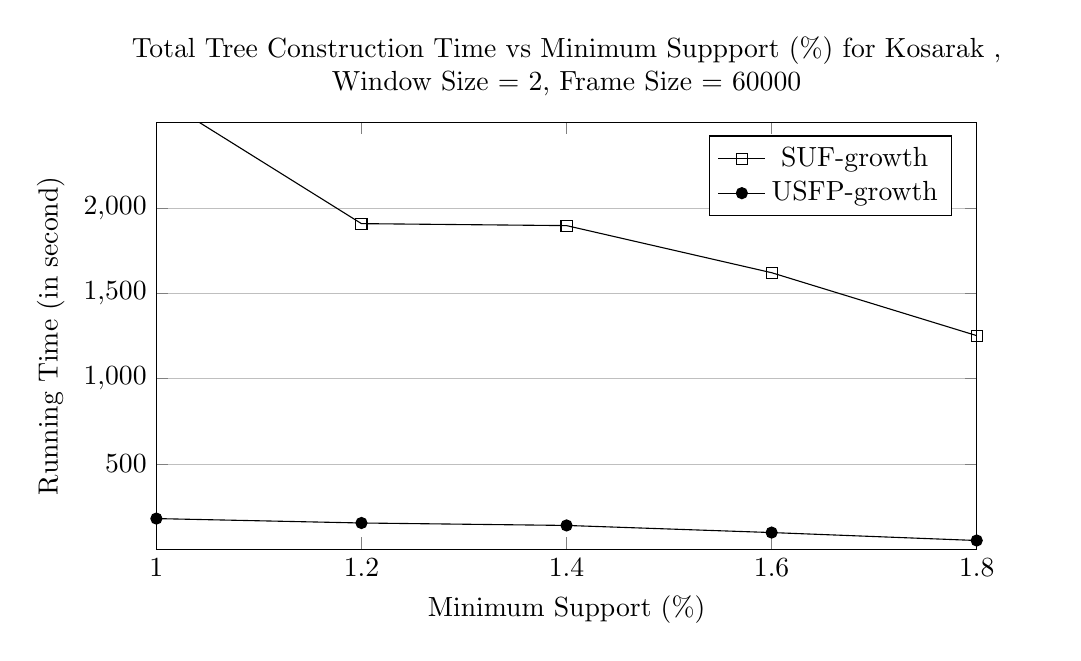
\begin{tikzpicture}
\begin{axis}[
	title={\parbox{\linewidth}{\centering Total Tree Construction Time vs Minimum Suppport (\%) for Kosarak , Window Size = 2, Frame Size = 60000}},
	width=12cm,
	height=7cm,
    xlabel={Minimum Support (\%) },
    ylabel={Running Time (in second)},
    xmin=1.0, xmax=1.8,
    ymin=0, ymax=2500,
    xtick={1.0,1.2,1.4,1.6,1.8},
    ytick={500,1000,1500,2000},
    legend pos=north east,
    ymajorgrids=true,
    grid style={line width=.2pt,draw=gray!50},
]
 
\addplot[
    solid, every mark/.append style={solid, fill=gray}, mark=square
    ]
    coordinates {
		(1.0 ,	2658.345	)
		(1.2,	1908.075	)
		(1.4,	1896.467	)
		(1.6,	1620.51		)
		(1.8,	1251.685	)	
		
	};
    \addlegendentry{SUF-growth}
\addplot[
    solid, every mark/.append style={solid, fill=black}, mark=*
    ]
    coordinates {
		(1.0  ,	179.797	)
		(1.2,	153.960	)
		(1.4,	139.599	)
		(1.6,	97.878	)
		(1.8,	51.297	)

};
    \addlegendentry{USFP-growth}
 
\end{axis}
\end{tikzpicture}
%\end{document}
            \caption{Total Tree Construction Time vs Minimum Support (\%) for Kosarak Dataset }
            \label{result:g_k_tree_construction_total}
            \end{figure}
            
            \begin{figure}[h]
            \centering
                %%mark = star, diamond, square, otimes
%\documentclass{article}
%\usepackage{pgfplots}
%\usepackage[justification=centering]{caption}
%\pgfplotsset{compat=newest}
%\begin{document}
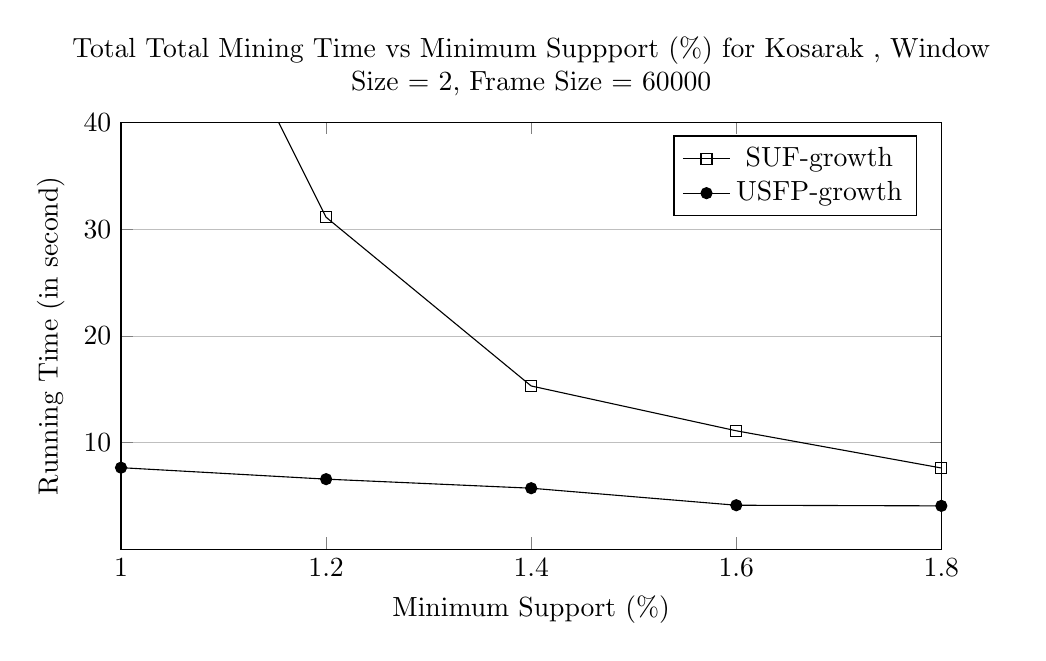
\begin{tikzpicture}
\begin{axis}[
	title={\parbox{\linewidth}{\centering Total Total Mining Time vs Minimum Suppport (\%) for Kosarak , Window Size = 2, Frame Size = 60000}},
	width=12cm,
	height=7cm,
    xlabel={Minimum Support (\%) },
    ylabel={Running Time (in second)},
    xmin=1.0, xmax=1.8,
    ymin=0, ymax=40,
    xtick={1.0,1.2,1.4,1.6,1.8},
    ytick={10,20,30,40},
    legend pos=north east,
    ymajorgrids=true,
    grid style={line width=.2pt,draw=gray!50},
]
 
\addplot[
    solid, every mark/.append style={solid, fill=gray}, mark=square
    ]
    coordinates {
		(1.0  ,	69.55)
		(1.2,	31.13)
		(1.4,	15.310)
		(1.6,	11.108)
		(1.8,	7.620)
};
    \addlegendentry{SUF-growth}
\addplot[
    solid, every mark/.append style={solid, fill=black}, mark=*
    ]
    coordinates {
		(1.0 ,	7.650	)
		(1.2,	6.575	)
		(1.4,	5.725	)
		(1.6,	4.128	)
		(1.8,	4.069	)
};
    \addlegendentry{USFP-growth}
 
\end{axis}
\end{tikzpicture}
%\end{document}
            \caption{Total Tree Mining Time vs Minimum Support (\%) for Kosarak Dataset }
            \label{result:g_k_mining_total}
            \end{figure}

            \begin{figure}[h]
            \centering
                %%mark = star, diamond, square, otimes
%\documentclass{article}
%\usepackage{pgfplots}
%\usepackage[justification=centering]{caption}
%\pgfplotsset{compat=newest}
%\begin{document}
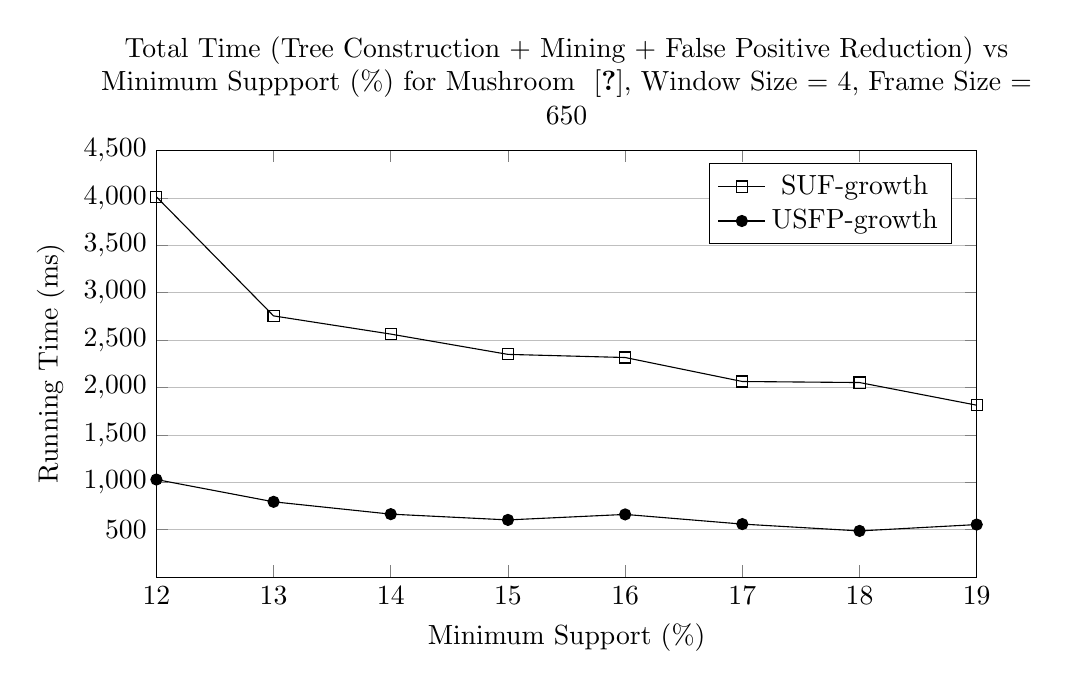
\begin{tikzpicture}
\begin{axis}[
	title={\parbox{\linewidth}{\centering Total Time (Tree Construction + Mining + False Positive Reduction) vs Minimum Suppport (\%) for Mushroom ~\cite{dataset}, Window Size = 4, Frame Size = 650}},
	width=12cm,
	height=7cm,
    xlabel={Minimum Support (\%) },
    ylabel={Running Time (ms)},
    xmin=12, xmax=19,
    ymin=0, ymax=4500,
    xtick={12,13,14,15,16,17,18,19},
    ytick={500,1000,1500,2000,2500,3000,3500,4000,4500},
    legend pos=north east,
    ymajorgrids=true,
    grid style={line width=.2pt,draw=gray!50},
]
 
\addplot[
    solid, every mark/.append style={solid, fill=gray}, mark=square
    ]
    coordinates {
	(12,4011)
	(13,2755)
	(14,2563)
	(15,2349)
	(16,2316)
	(17,2063)
	(18,2052)
	(19,1813)
};
    \addlegendentry{SUF-growth}
\addplot[
    solid, every mark/.append style={solid, fill=black}, mark=*
    ]
    coordinates {
	(12,1029)
	(13,794)
	(14,664)
	(15,603)
	(16,661)
	(17,559)
	(18,487)
	(19,554)
};
    \addlegendentry{USFP-growth}
 
\end{axis}
\end{tikzpicture}
%\end{document}
            \caption{Runtime vs Minimum Support (\%) for Kosarak Dataset }
            \label{result:g_k_total}
            \end{figure}
            
\clearpage
    \subsubsection{Memory Comparison}
        As our proposed \emph{US-tree} have the capability to share nodes more than \emph{SUF-growth}, we get much more gain in memory. The experimental result also indicates that very clearly. Figure-\ref{result:g_m_memory_node} shows the memory comparison on mushroom dataset. Mushroom is the dense database so we get  much more gain in memory. The graph clearly shows that with the increase of total transaction in the tree gives the much more gain. For chess dataset the compactness of tree is also very impressive as this dataset is also compact (figure-\ref{result:g_chess_memory_node}) the Dense dataset have more scope to share nodes more. Figure-\ref{result:g_t10_memory_node} also shows that in T40I10D100K database we also gain the memory optimization. Figure-\ref{result:g_k_memory_node} shows memory comparison between \emph{USFP-growth} vs \emph{SUF-growth} ~\cite{suf_growth}. On this sparse database it has been clearly shown that, lot of memory optimization has been possible with our proposed algorithm. As the database is sparse, we get the memory gain less then dense one.
            \begin{figure}[h]
            \centering
                %mark = star, diamond, square, otimes
%\documentclass{article}
%\usepackage{pgfplots}
%\usepackage[justification=centering]{caption}
%\pgfplotsset{compat=newest}
%\begin{document}
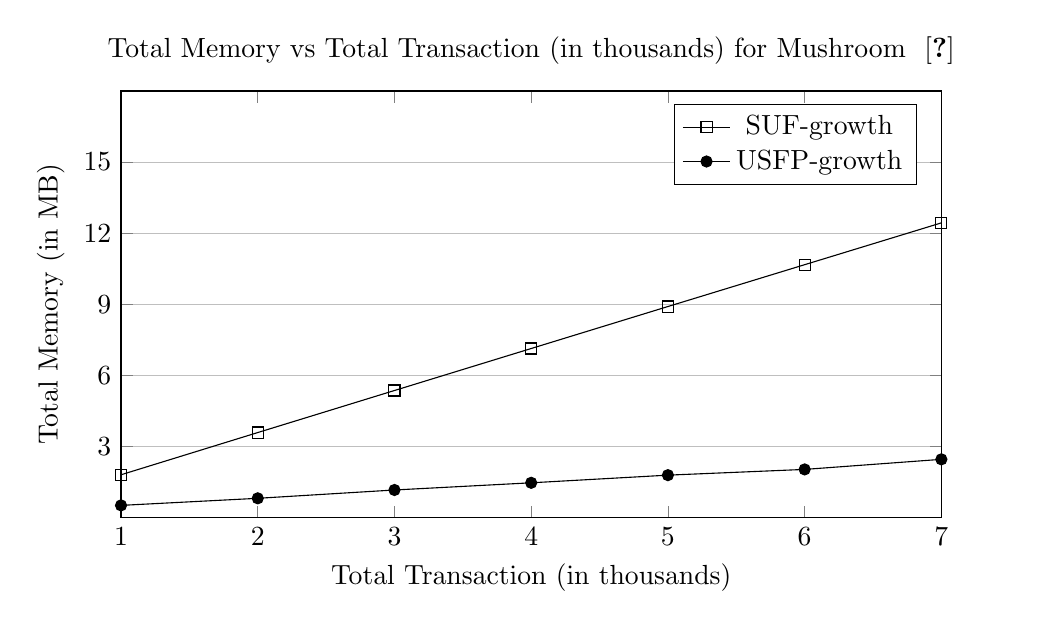
\begin{tikzpicture}
\begin{axis}[
	title={\parbox{\linewidth}{\centering Total Memory vs Total Transaction (in thousands) for Mushroom ~\cite{dataset}}},
	width=12cm,
	height=7cm,
    xlabel={Total Transaction (in thousands) },
    ylabel={Total Memory (in MB) },
    xmin=1, xmax=7,
    ymin=0, ymax=18,
    xtick={1,2,3,4,5,6,7},
    ytick={3,6,9,12,15},
    legend pos=north east,
    ymajorgrids=true,
    grid style={line width=.2pt,draw=gray!50},
]
 
\addplot[
    solid, every mark/.append style={solid, fill=gray}, mark=square
    ]
    coordinates {
			(1,1.807  )
			(2,3.588  )
			(3,5.362  )
			(4,7.134     )
			(5,8.905  )
			(6,10.670 )
			(7,12.434  )



	};
    \addlegendentry{SUF-growth}
\addplot[
    solid, every mark/.append style={solid, fill=black}, mark=*
    ]
    coordinates {
			(1,.5152  )
			(2,.814  )
			(3,1.165 )
			(4,1.468 )
			(5,1.791  )
			(6,2.033 )
			(7,2.458 )


};
    \addlegendentry{USFP-growth}
 
\end{axis}
\end{tikzpicture}
%\end{document}
            \caption{Total Memory vs Total Transaction (in thousand) for Mushroom Dataset }
            \label{result:g_m_memory_node}
            \end{figure}
            
            \begin{figure}[h]
            \centering
                %mark = star, diamond, square, otimes
%\documentclass{article}
%\usepackage{pgfplots}
%\usepackage[justification=centering]{caption}
%\pgfplotsset{compat=newest}
%\begin{document}
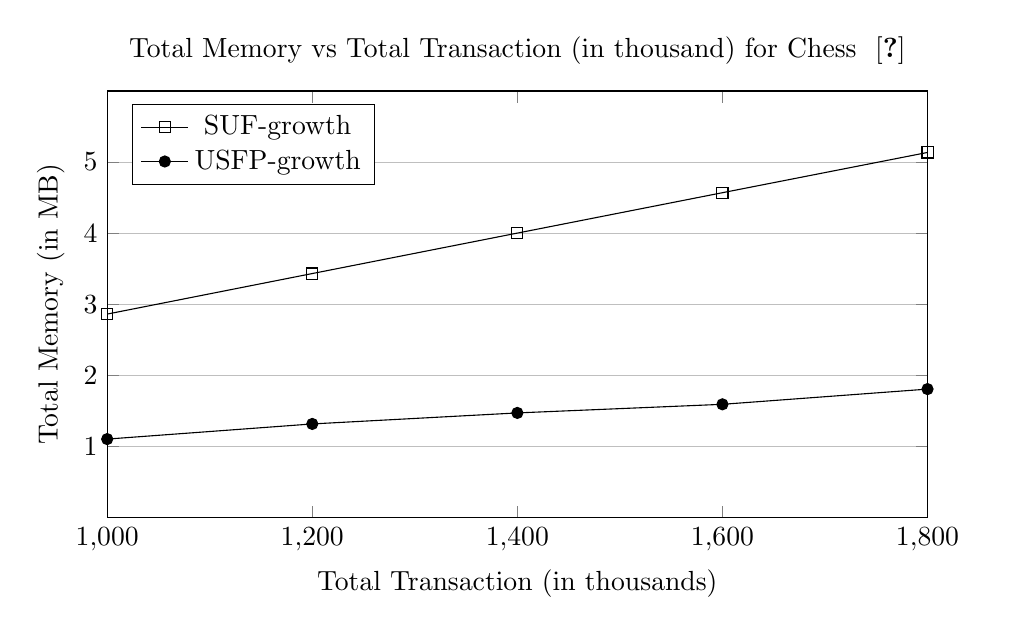
\begin{tikzpicture}
\begin{axis}[
	title={\parbox{\linewidth}{\centering Total Memory vs Total Transaction (in thousand) for Chess ~\cite{dataset}}},
	width=12cm,
	height=7cm,
    xlabel={Total Transaction (in thousands) },
    ylabel={Total Memory (in MB) },
    xmin=1000, xmax=1800,
    ymin=0, ymax=6,
    xtick={600,800,1000,1200,1400,1600,1800},
    ytick={1,2,3,4,5},
    legend pos=north west,
    ymajorgrids=true,
    grid style={line width=.2pt,draw=gray!50},
]
 
\addplot[
    solid, every mark/.append style={solid, fill=gray}, mark=square
    ]
    coordinates {
			(600,	1.720)
			(800,	2.291)
			(1000,	2.862)
			(1200,	3.432)
			(1400,	4.001)
			(1600,	4.569)
            (1800,	5.135)



	};
    \addlegendentry{SUF-growth}
\addplot[
    solid, every mark/.append style={solid, fill=black}, mark=*
    ]
    coordinates {
			(600,	0.681 )
			(800,	0.865 )
			(1000,	1.104 )
			(1200,	1.317 )
			(1400,	1.472 )
			(1600,	1.593 )
            (1800,	1.807 )


};
    \addlegendentry{USFP-growth}
 
\end{axis}
\end{tikzpicture}
%\end{document}
            \caption{Total Memory vs Total Transaction (in thousand) for Chess Dataset }
            \label{result:g_chess_memory_node}
            \end{figure}
            
            \begin{figure}[h]
                %%%mark = star, diamond, square, otimes
%\documentclass{article}
%\usepackage{pgfplots}
%\usepackage[justification=centering]{caption}
%\pgfplotsset{compat=newest}
%\begin{document}
\begin{figure}
\centering

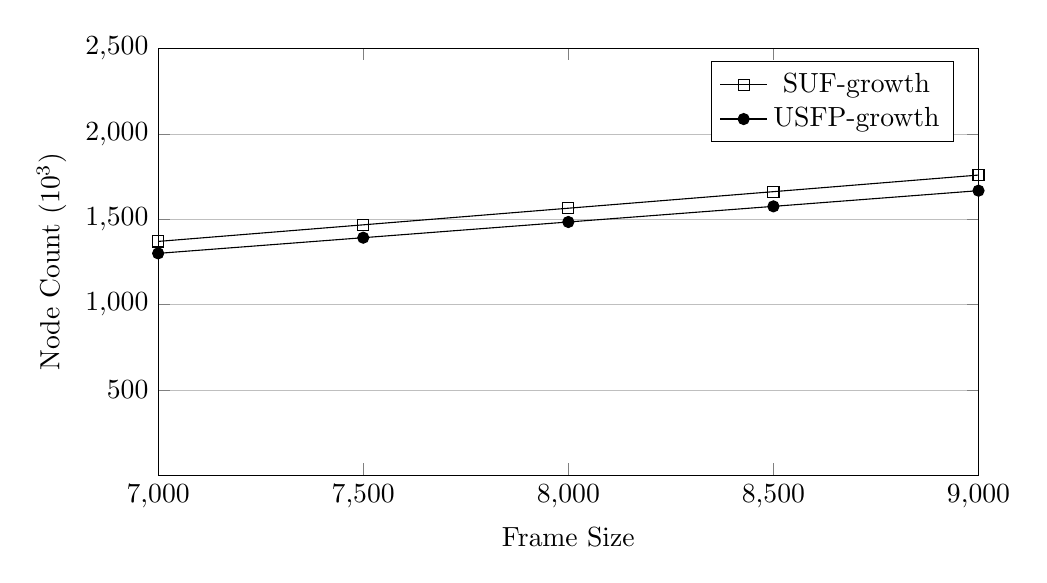
\begin{tikzpicture}
\begin{axis}[
 width=12cm,
   height=7cm,
    xlabel={Frame Size },
    ylabel={Node Count ($10^3$)},
    xmin=7000, xmax=9000,
    ymin=0, ymax=2500,
    xtick={7000,7500,8000,8500,9000},
    ytick={500,1000,1500,2000,2500},
    legend pos=north east,
    ymajorgrids=true,
    grid style={line width=.2pt,draw=gray!50},
]
 
\addplot[
    solid, every mark/.append style={solid, fill=gray}, mark=square
    ]
    coordinates {
			(7000,1369.555 )
			(7500,1466.766 )
			(8000,1564.122 )
			(8500,1661.100 )
			(9000,1758.412 )
			(9500,1855.734 )

	};
    \addlegendentry{SUF-growth}
\addplot[
    solid, every mark/.append style={solid, fill=black}, mark=*
    ]
    coordinates {
					(7000,1299.510)
		(7500,1391.388)
		(8000,1483.378)
		(8500,1574.984)
		(9000,1666.912)
		(9500,1758.773)

};
    \addlegendentry{USFP-growth}
 
\end{axis}
\end{tikzpicture}
\caption{Total Tree Node vs Frame Size (Window Size = 5) for T40I10D100K database}
\label{result:t10_total_mem_node}
\end{figure}
%\end{document}
            \caption{Total Memory vs Total Transaction (in thousand) for T40I10D100K Dataset }
            \label{result:g_t10_memory_node}
            \end{figure}
        
            \begin{figure}[h]
            \centering
                %mark = star, diamond, square, otimes
%\documentclass{article}
%\usepackage{pgfplots}
%\usepackage[justification=centering]{caption}
%\pgfplotsset{compat=newest}
%\begin{document}
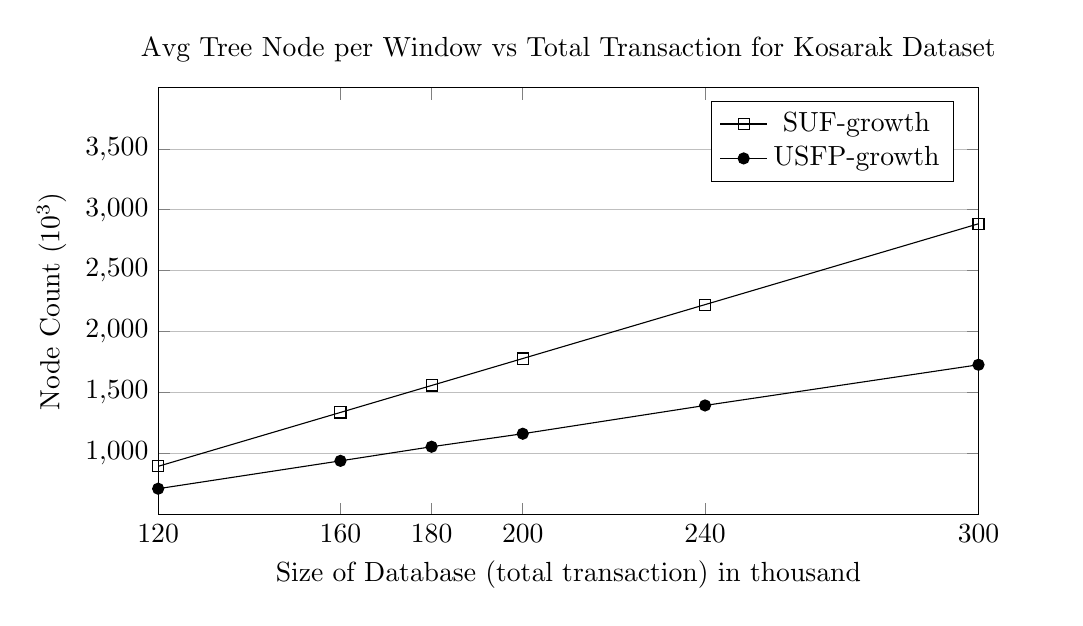
\begin{tikzpicture}
\begin{axis}[
	title={\parbox{\linewidth}{\centering Avg Tree Node per Window vs Total Transaction for Kosarak Dataset}},
	width=12cm,
	height=7cm,
    xlabel={Size of Database (total transaction) in thousand},
    ylabel={Node Count ($10^3$)},
    xmin=120, xmax=300,
    ymin=500, ymax=4000,
    xtick={120,160,180,200,240,300},
    ytick={1000,1500,2000,2500,3000,3500},
    legend pos=north east,
    ymajorgrids=true,
    grid style={line width=.2pt,draw=gray!50},
]
 
\addplot[
    solid, every mark/.append style={solid, fill=gray}, mark=square
    ]
    coordinates {
			(120,	895.299)
			(160,	1337.507)
			(180,	1558.611)
			(200,	1779.715)
			(240,	2221.923)
			(300,	2885.235)

	};
    \addlegendentry{SUF-growth}
\addplot[
    solid, every mark/.append style={solid, fill=black}, mark=*
    ]
    coordinates {
			(120,	711.772)
			(160,	940.241)
			(180,	1056.093)
			(200,	1162.692)
			(240,	1394.691)
			(300,	1728.543)


};
    \addlegendentry{USFP-growth}
 
\end{axis}
\end{tikzpicture}
%\end{document}
            \caption{Total Memory vs Total Transaction (in thousand) for Kosarak Dataset }
            \label{result:g_k_memory_node}
            \end{figure}